	\begin{figure}
			\centering
			\subfloat[SHREK]{
				\scalebox{.4}{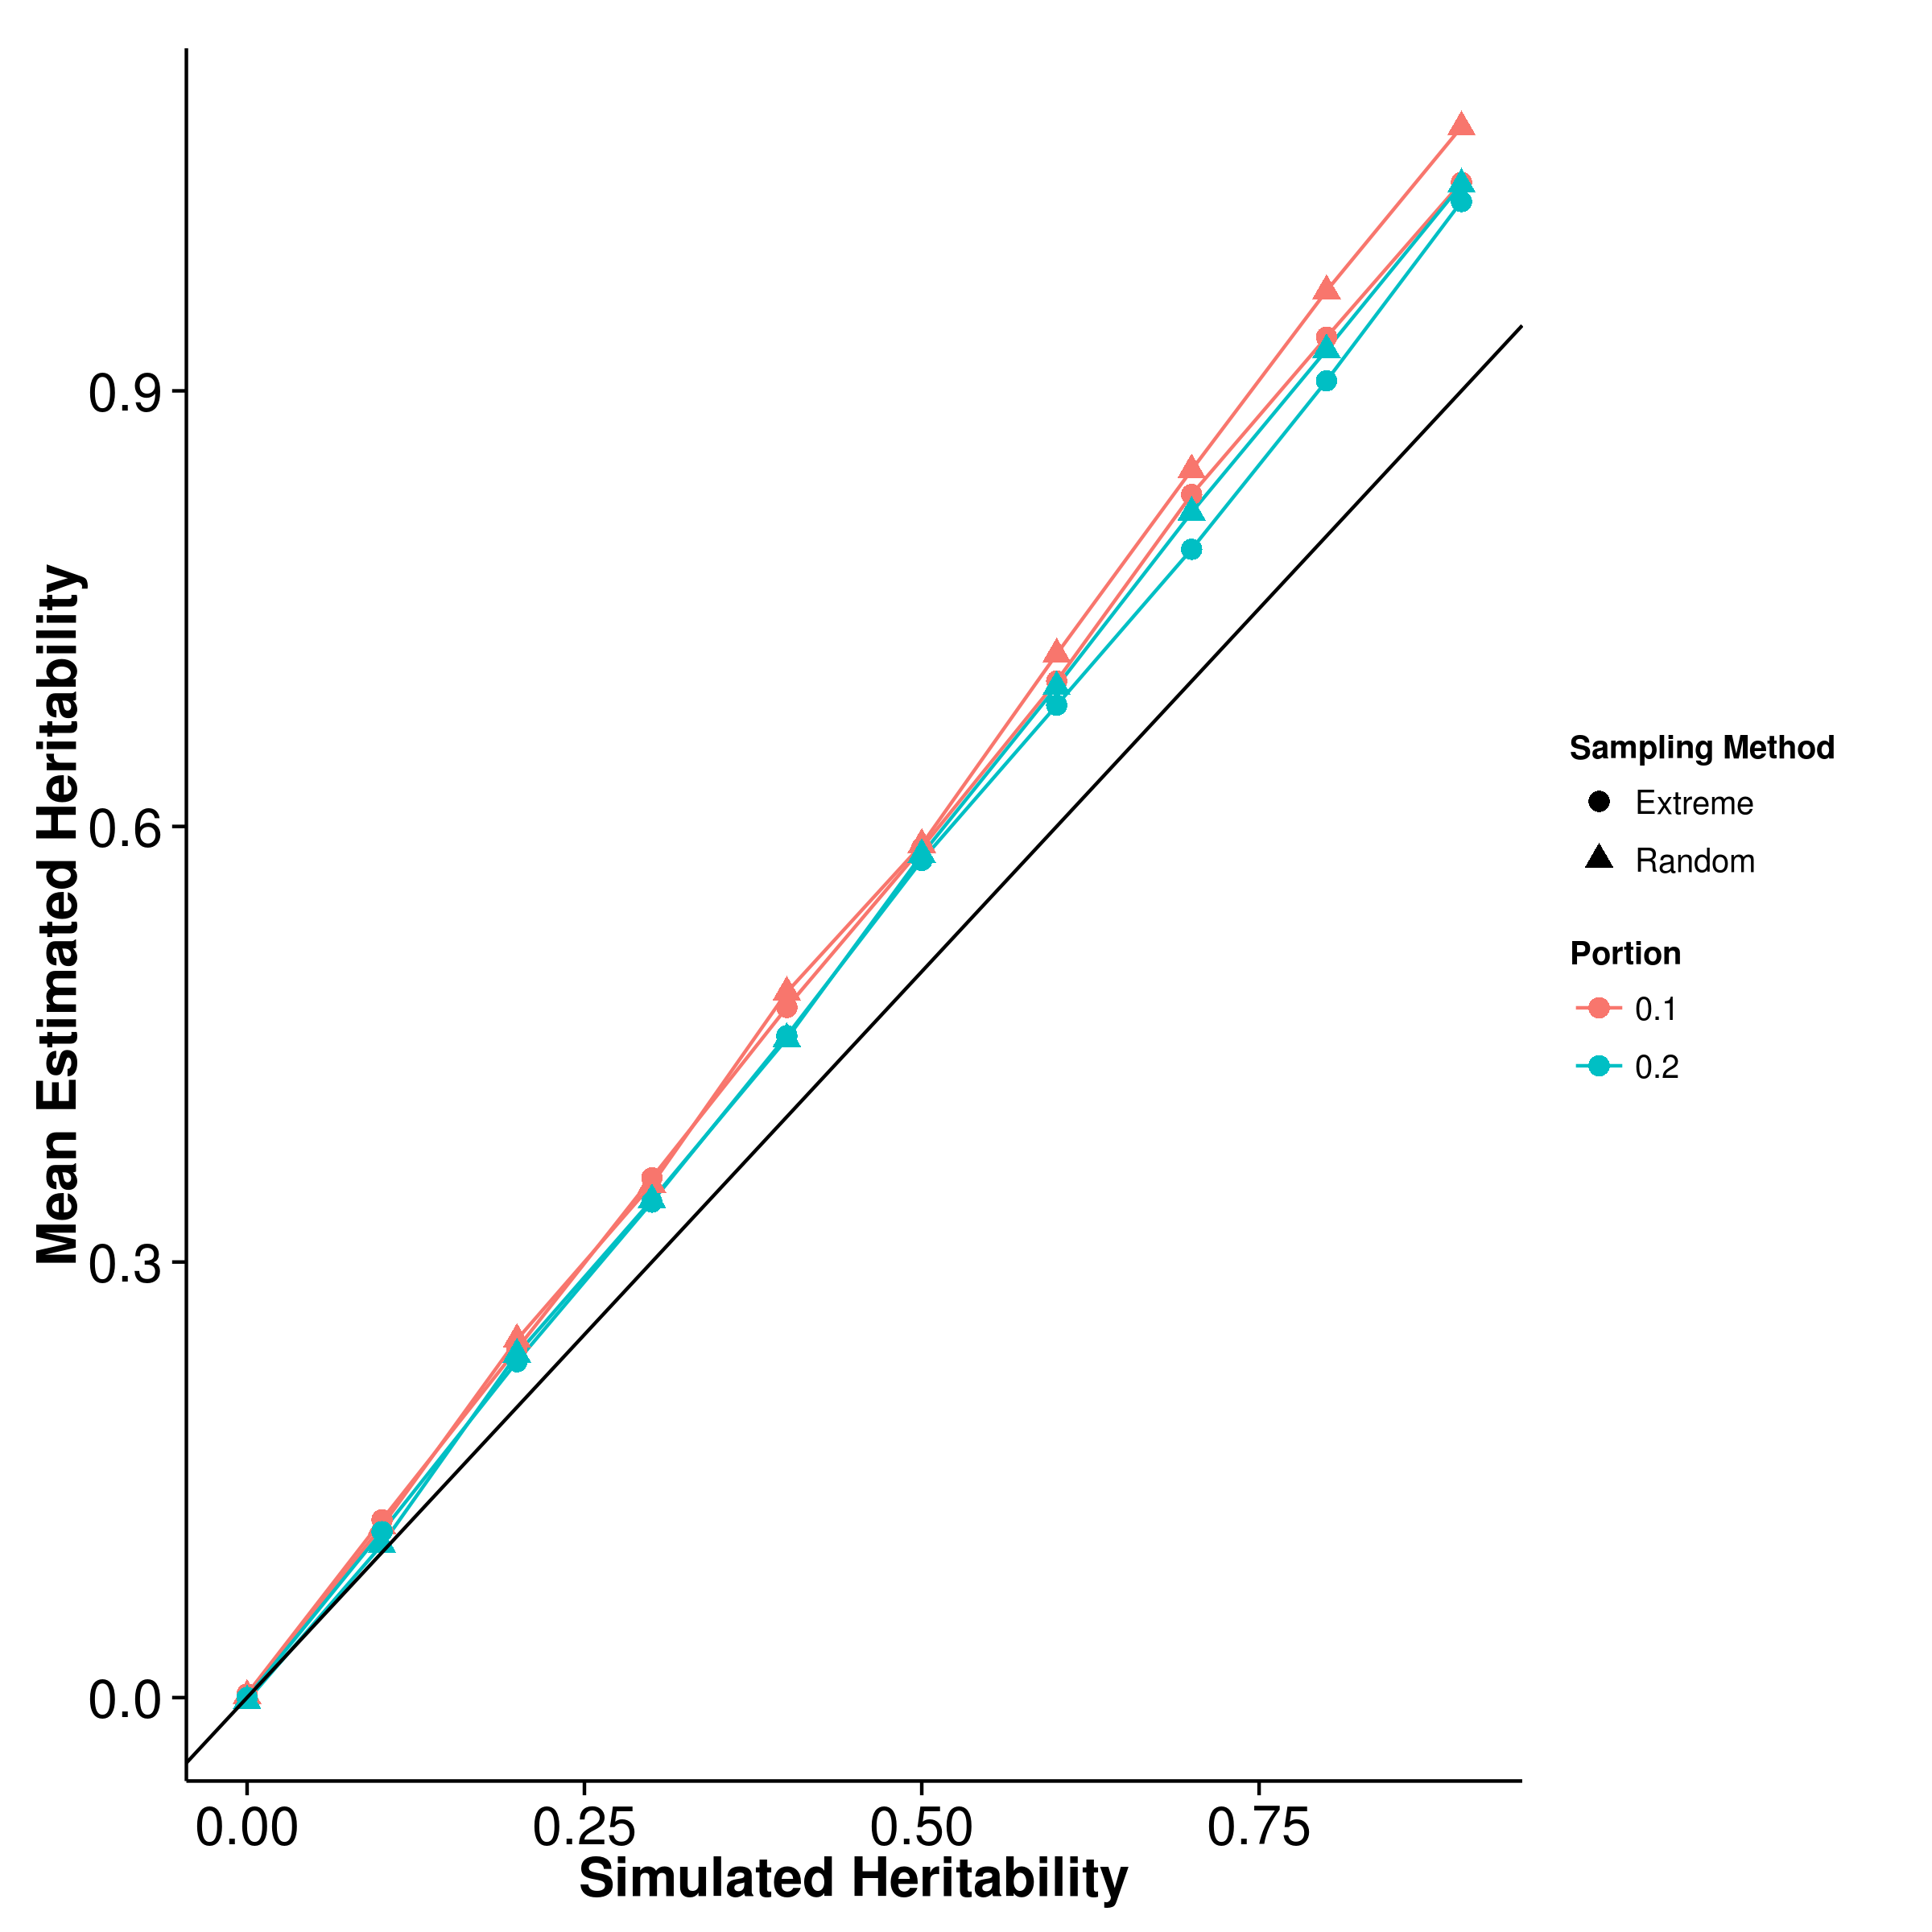
\includegraphics{figure/he_summary/pheno_extreme/shrek_extremeSelect_mean.png}}
				\label{fig:shrekExMean}
			}
			\subfloat[GCTA]{
				\scalebox{.4}{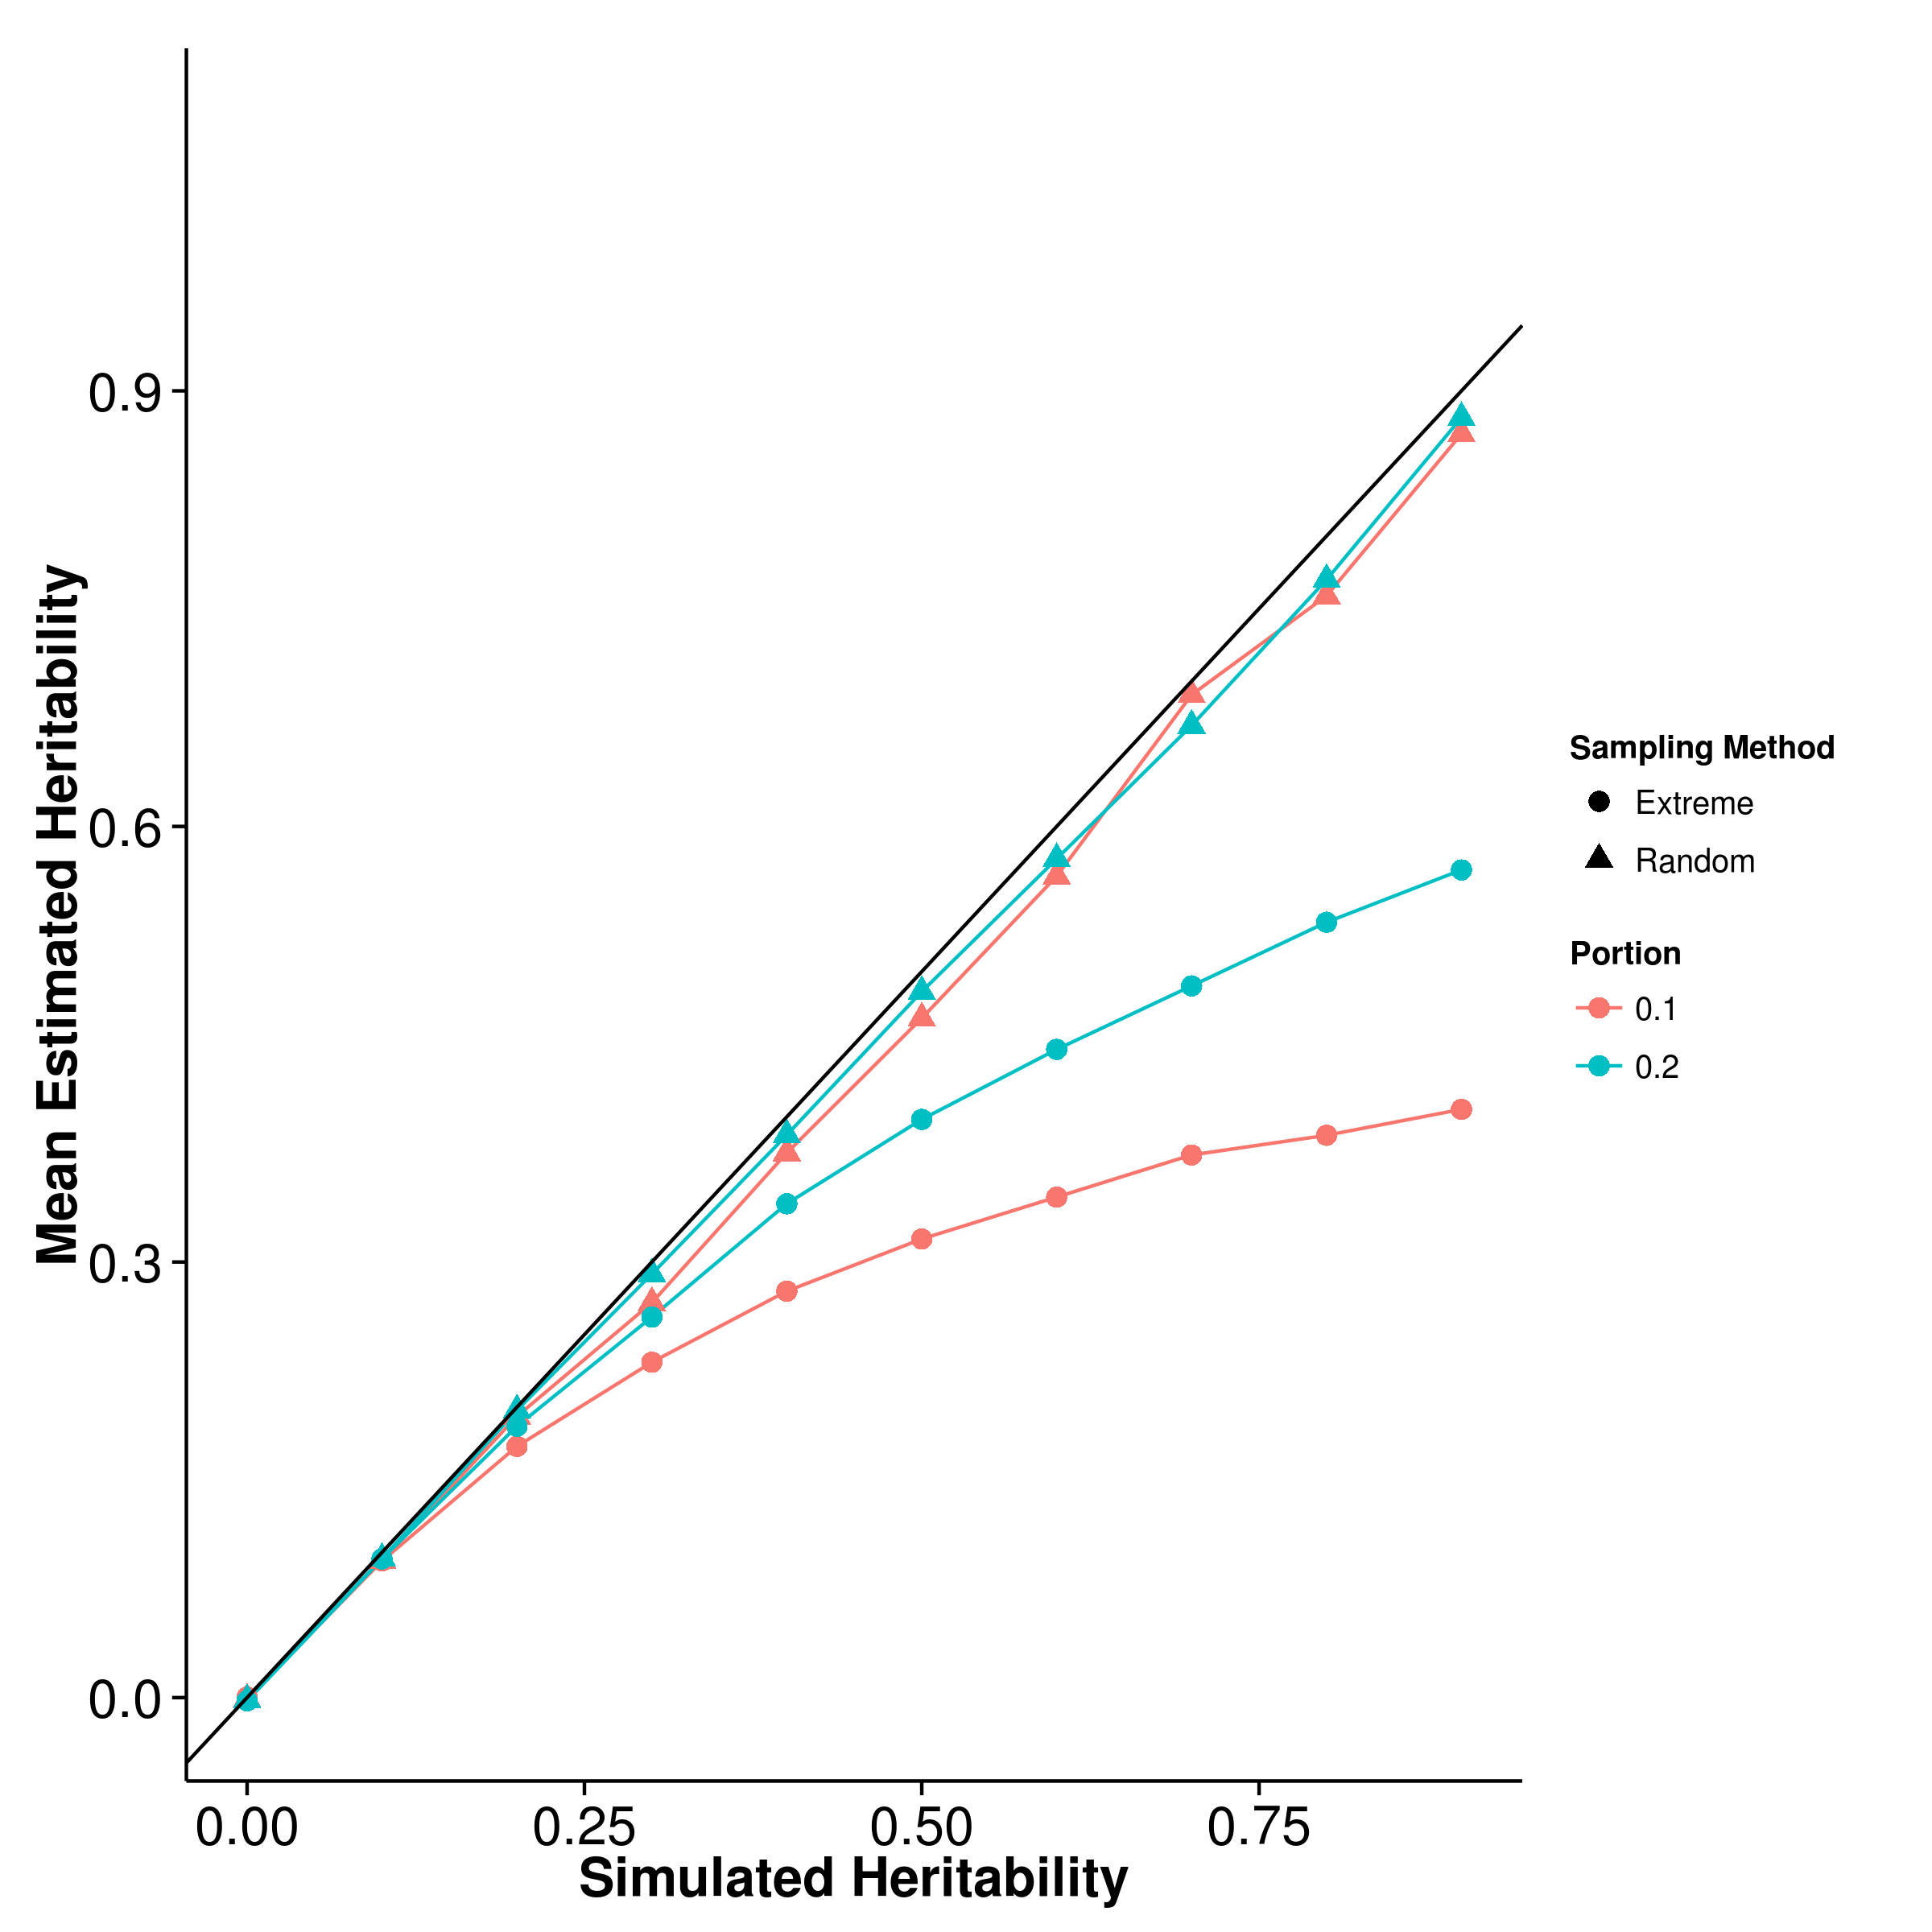
\includegraphics{figure/he_summary/pheno_extreme/gcta_extremeSelect_mean.png}}
				\label{fig:gctaExMean}
			}\\
			\subfloat[LDSC with fix intercept]{
				\scalebox{.4}{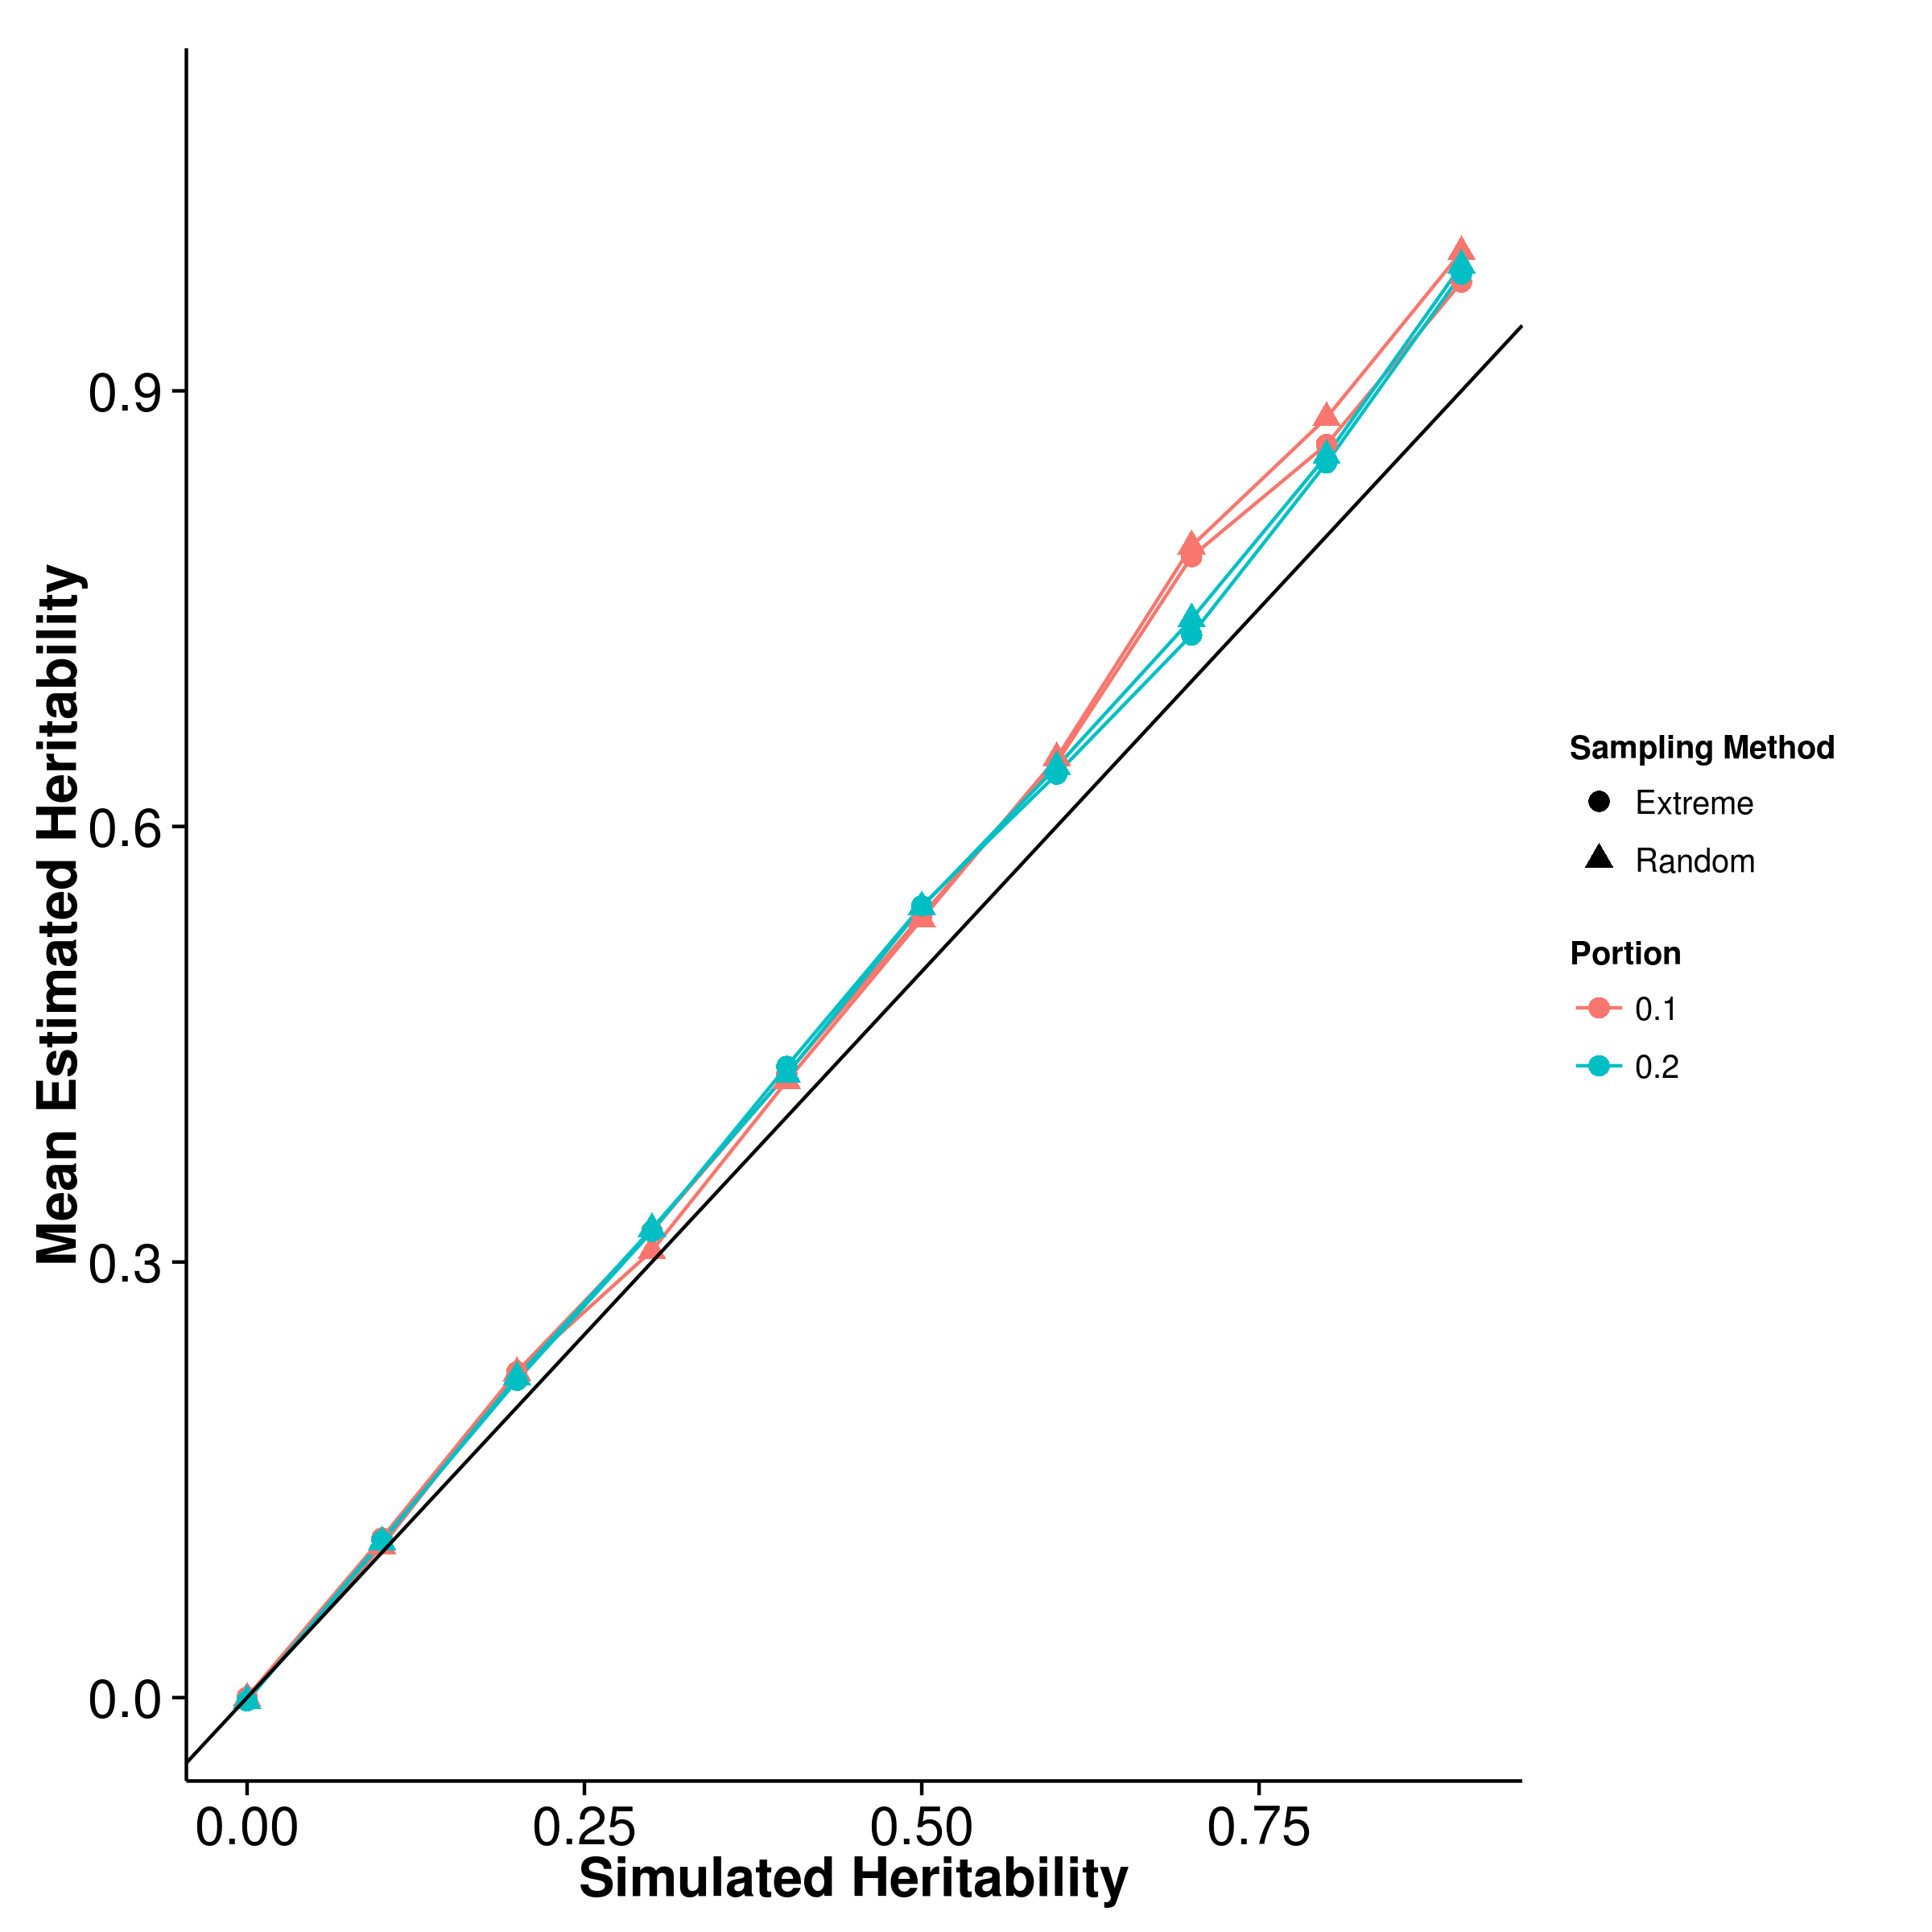
\includegraphics{figure/he_summary/pheno_extreme/ldsc_extremeSelect_mean.png}}
				\label{fig:ldscExMean}
			}
			\subfloat[LDSC with intercept estimation]{
				
				\scalebox{.4}{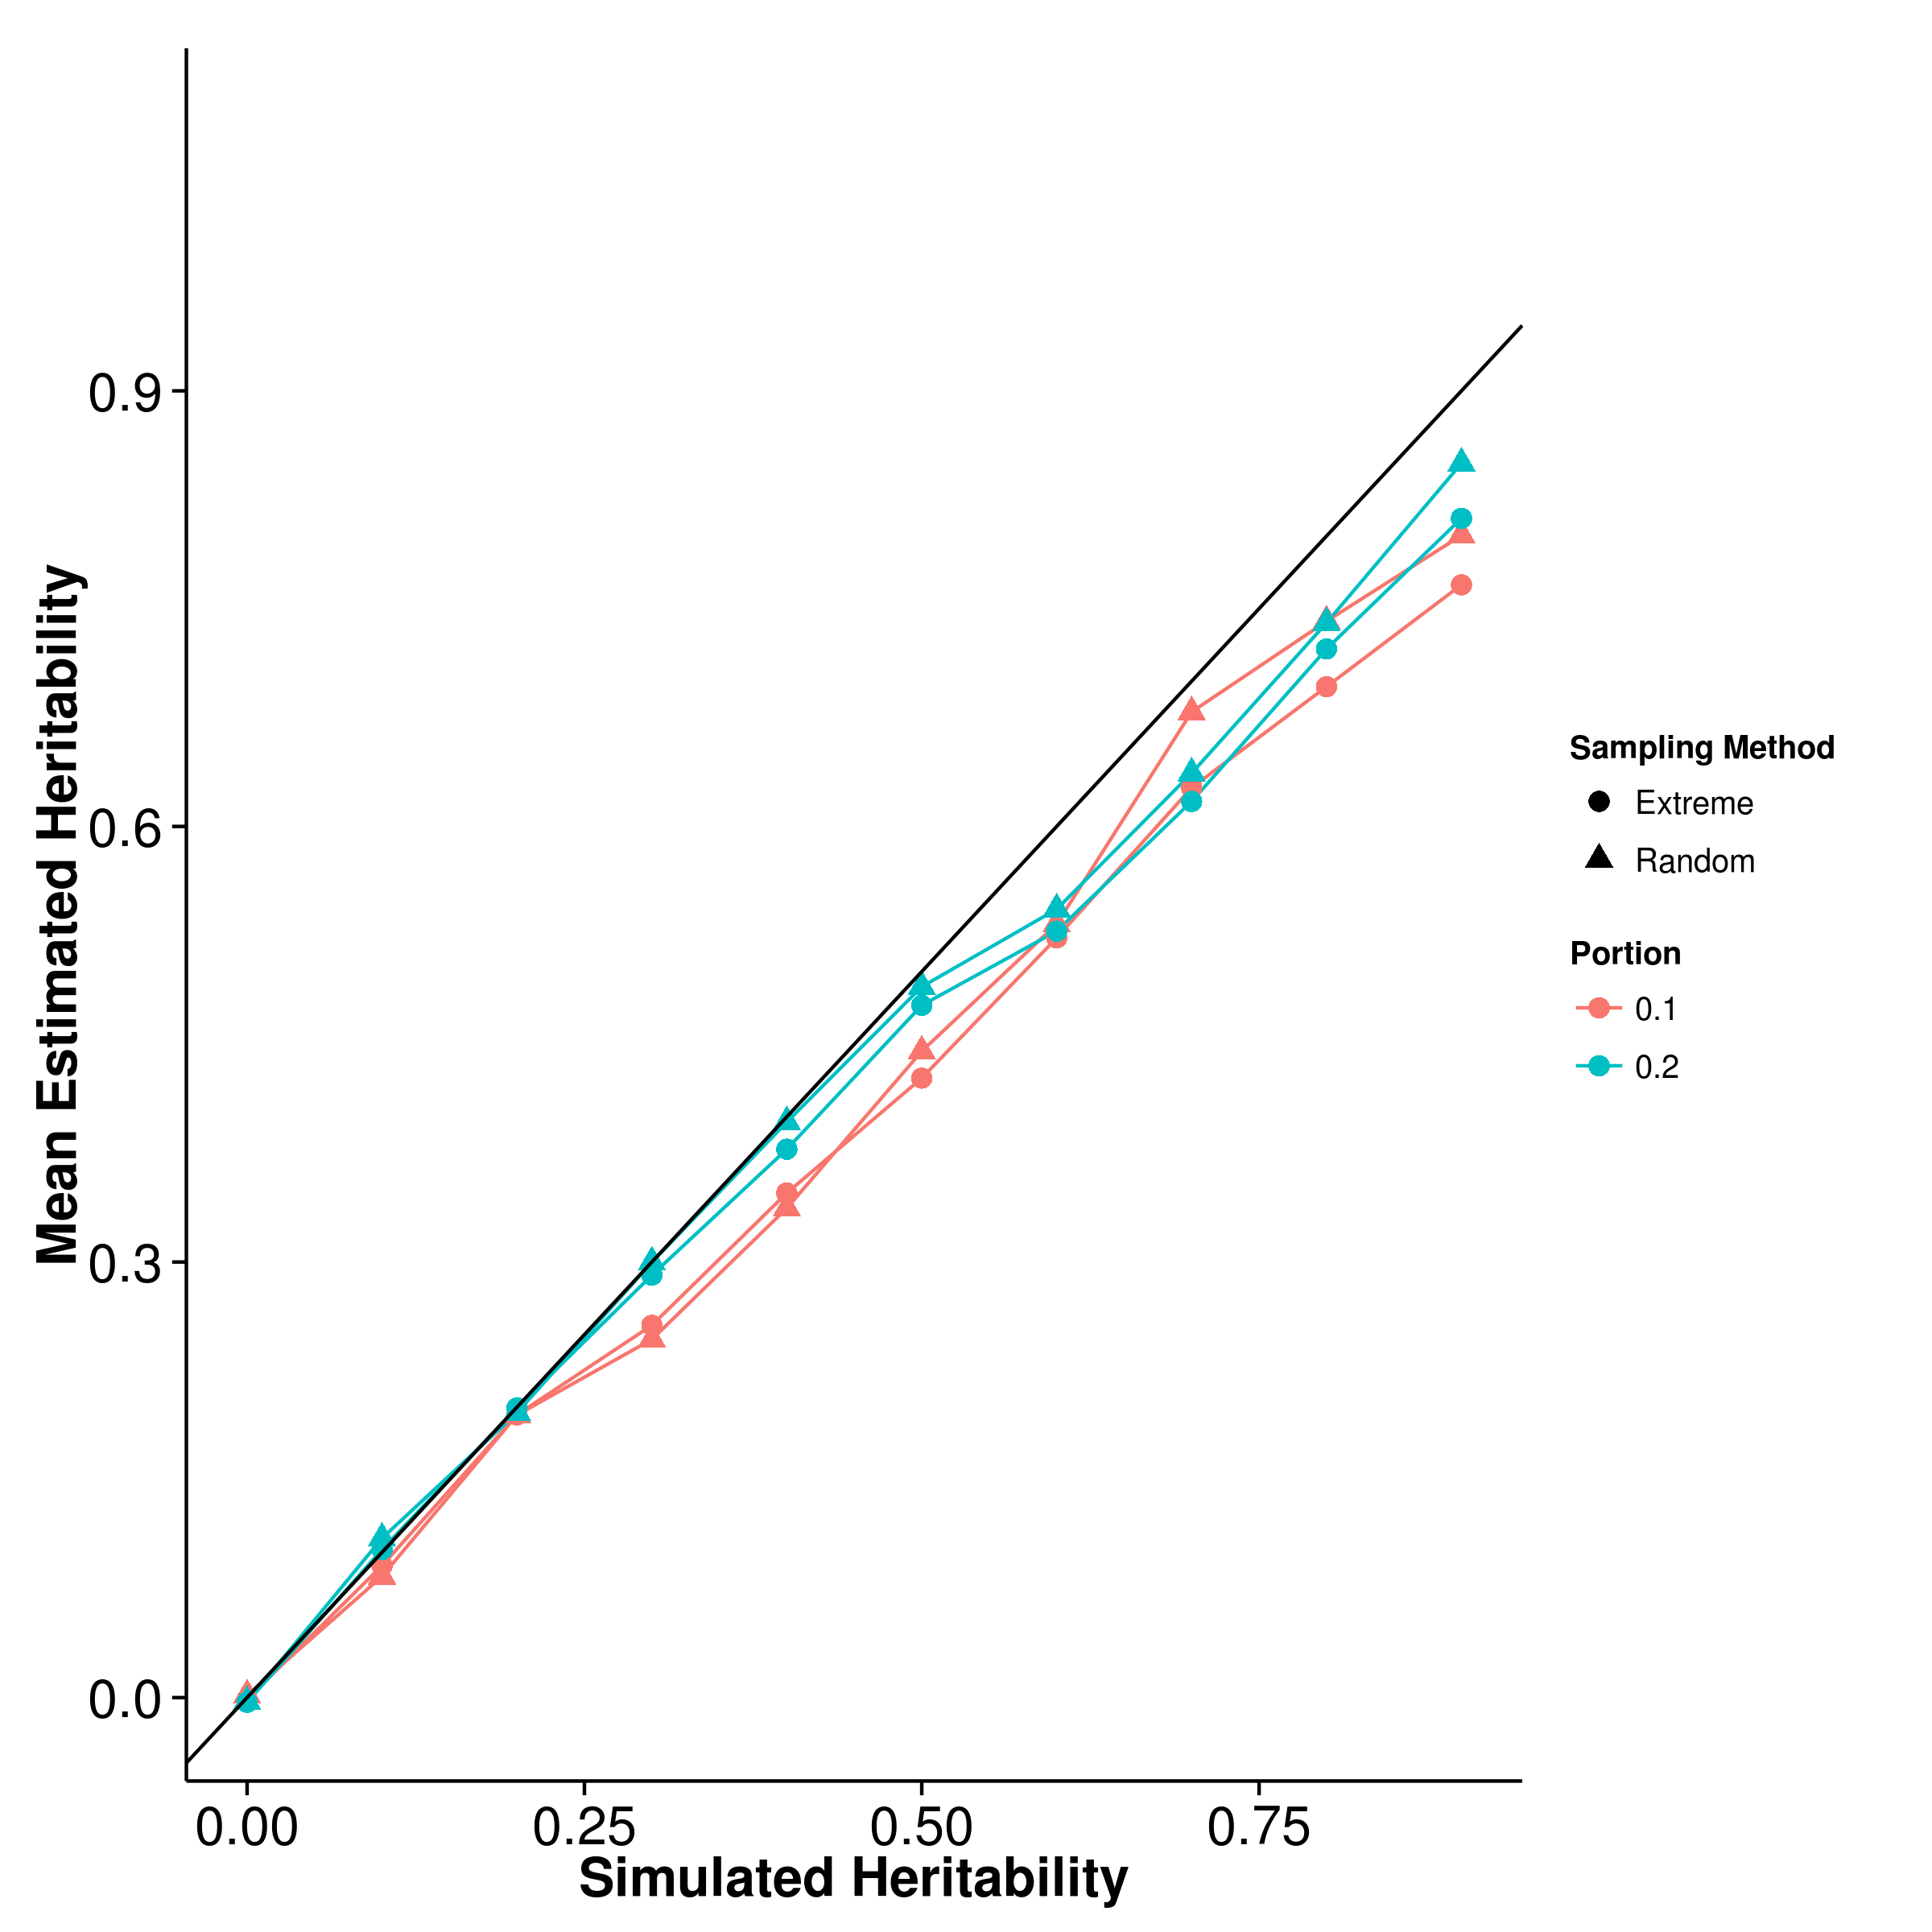
\includegraphics{figure/he_summary/pheno_extreme/ldscIn_extremeSelect_mean.png}}
				\label{fig:ldscInExMean}
			}
			\caption[Mean of Extreme Phenotype Selection Simulation Results]
			{Mean of results from extreme phenotype simulation.
				The performance of the algorithms when random sampling was performed were similar to what was observed in the quantitative trait simulation.
				However, when extreme phenotype was performed, a larger under estimation was observed for \gls{gcta} and it gets worst when the portion of sample selected decreases.
				On the other hand, the performance of \gls{shrek} and \gls{ldsc} under the extreme phenotype selection was similar to that from the random samplings.
				} 
			\label{fig:ExMean}
		\end{figure}
		
		\begin{figure}
			\centering
			\subfloat[SHREK]{
				\scalebox{.4}{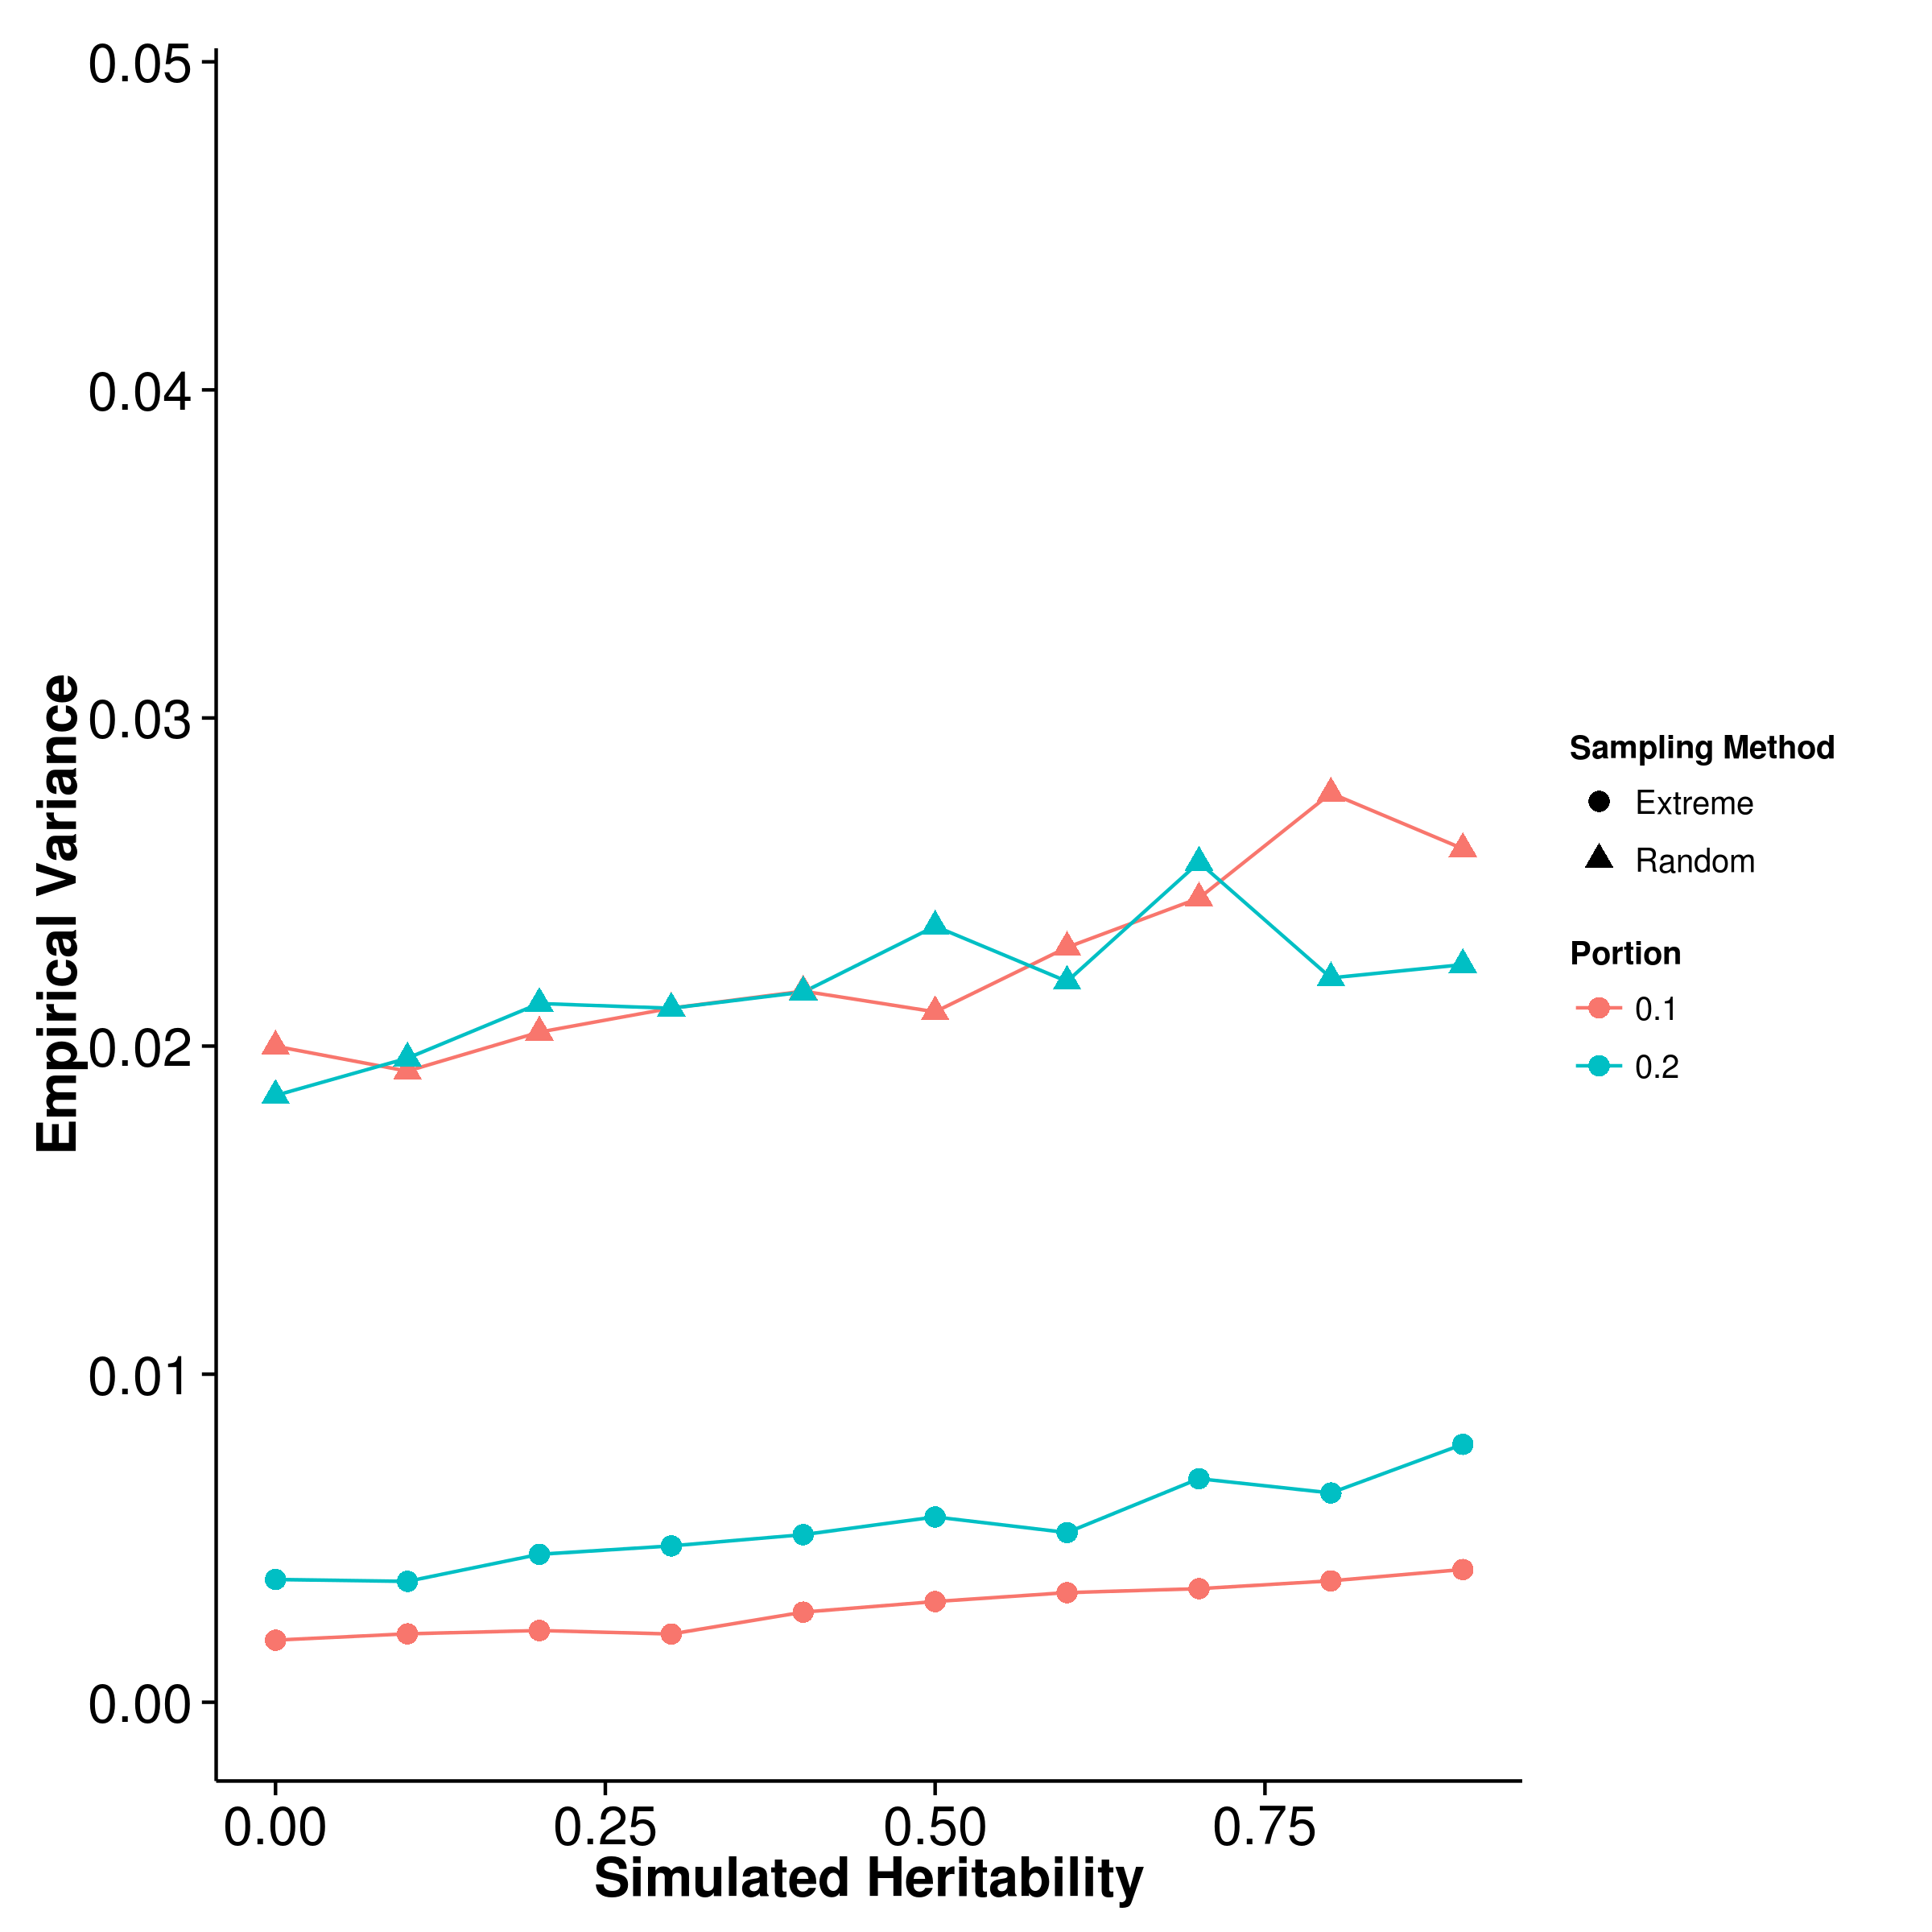
\includegraphics{figure/he_summary/pheno_extreme/shrek_extremeSelect_var.png}}
				\label{fig:shrekExVar}
			}
			\subfloat[GCTA]{
				\scalebox{.4}{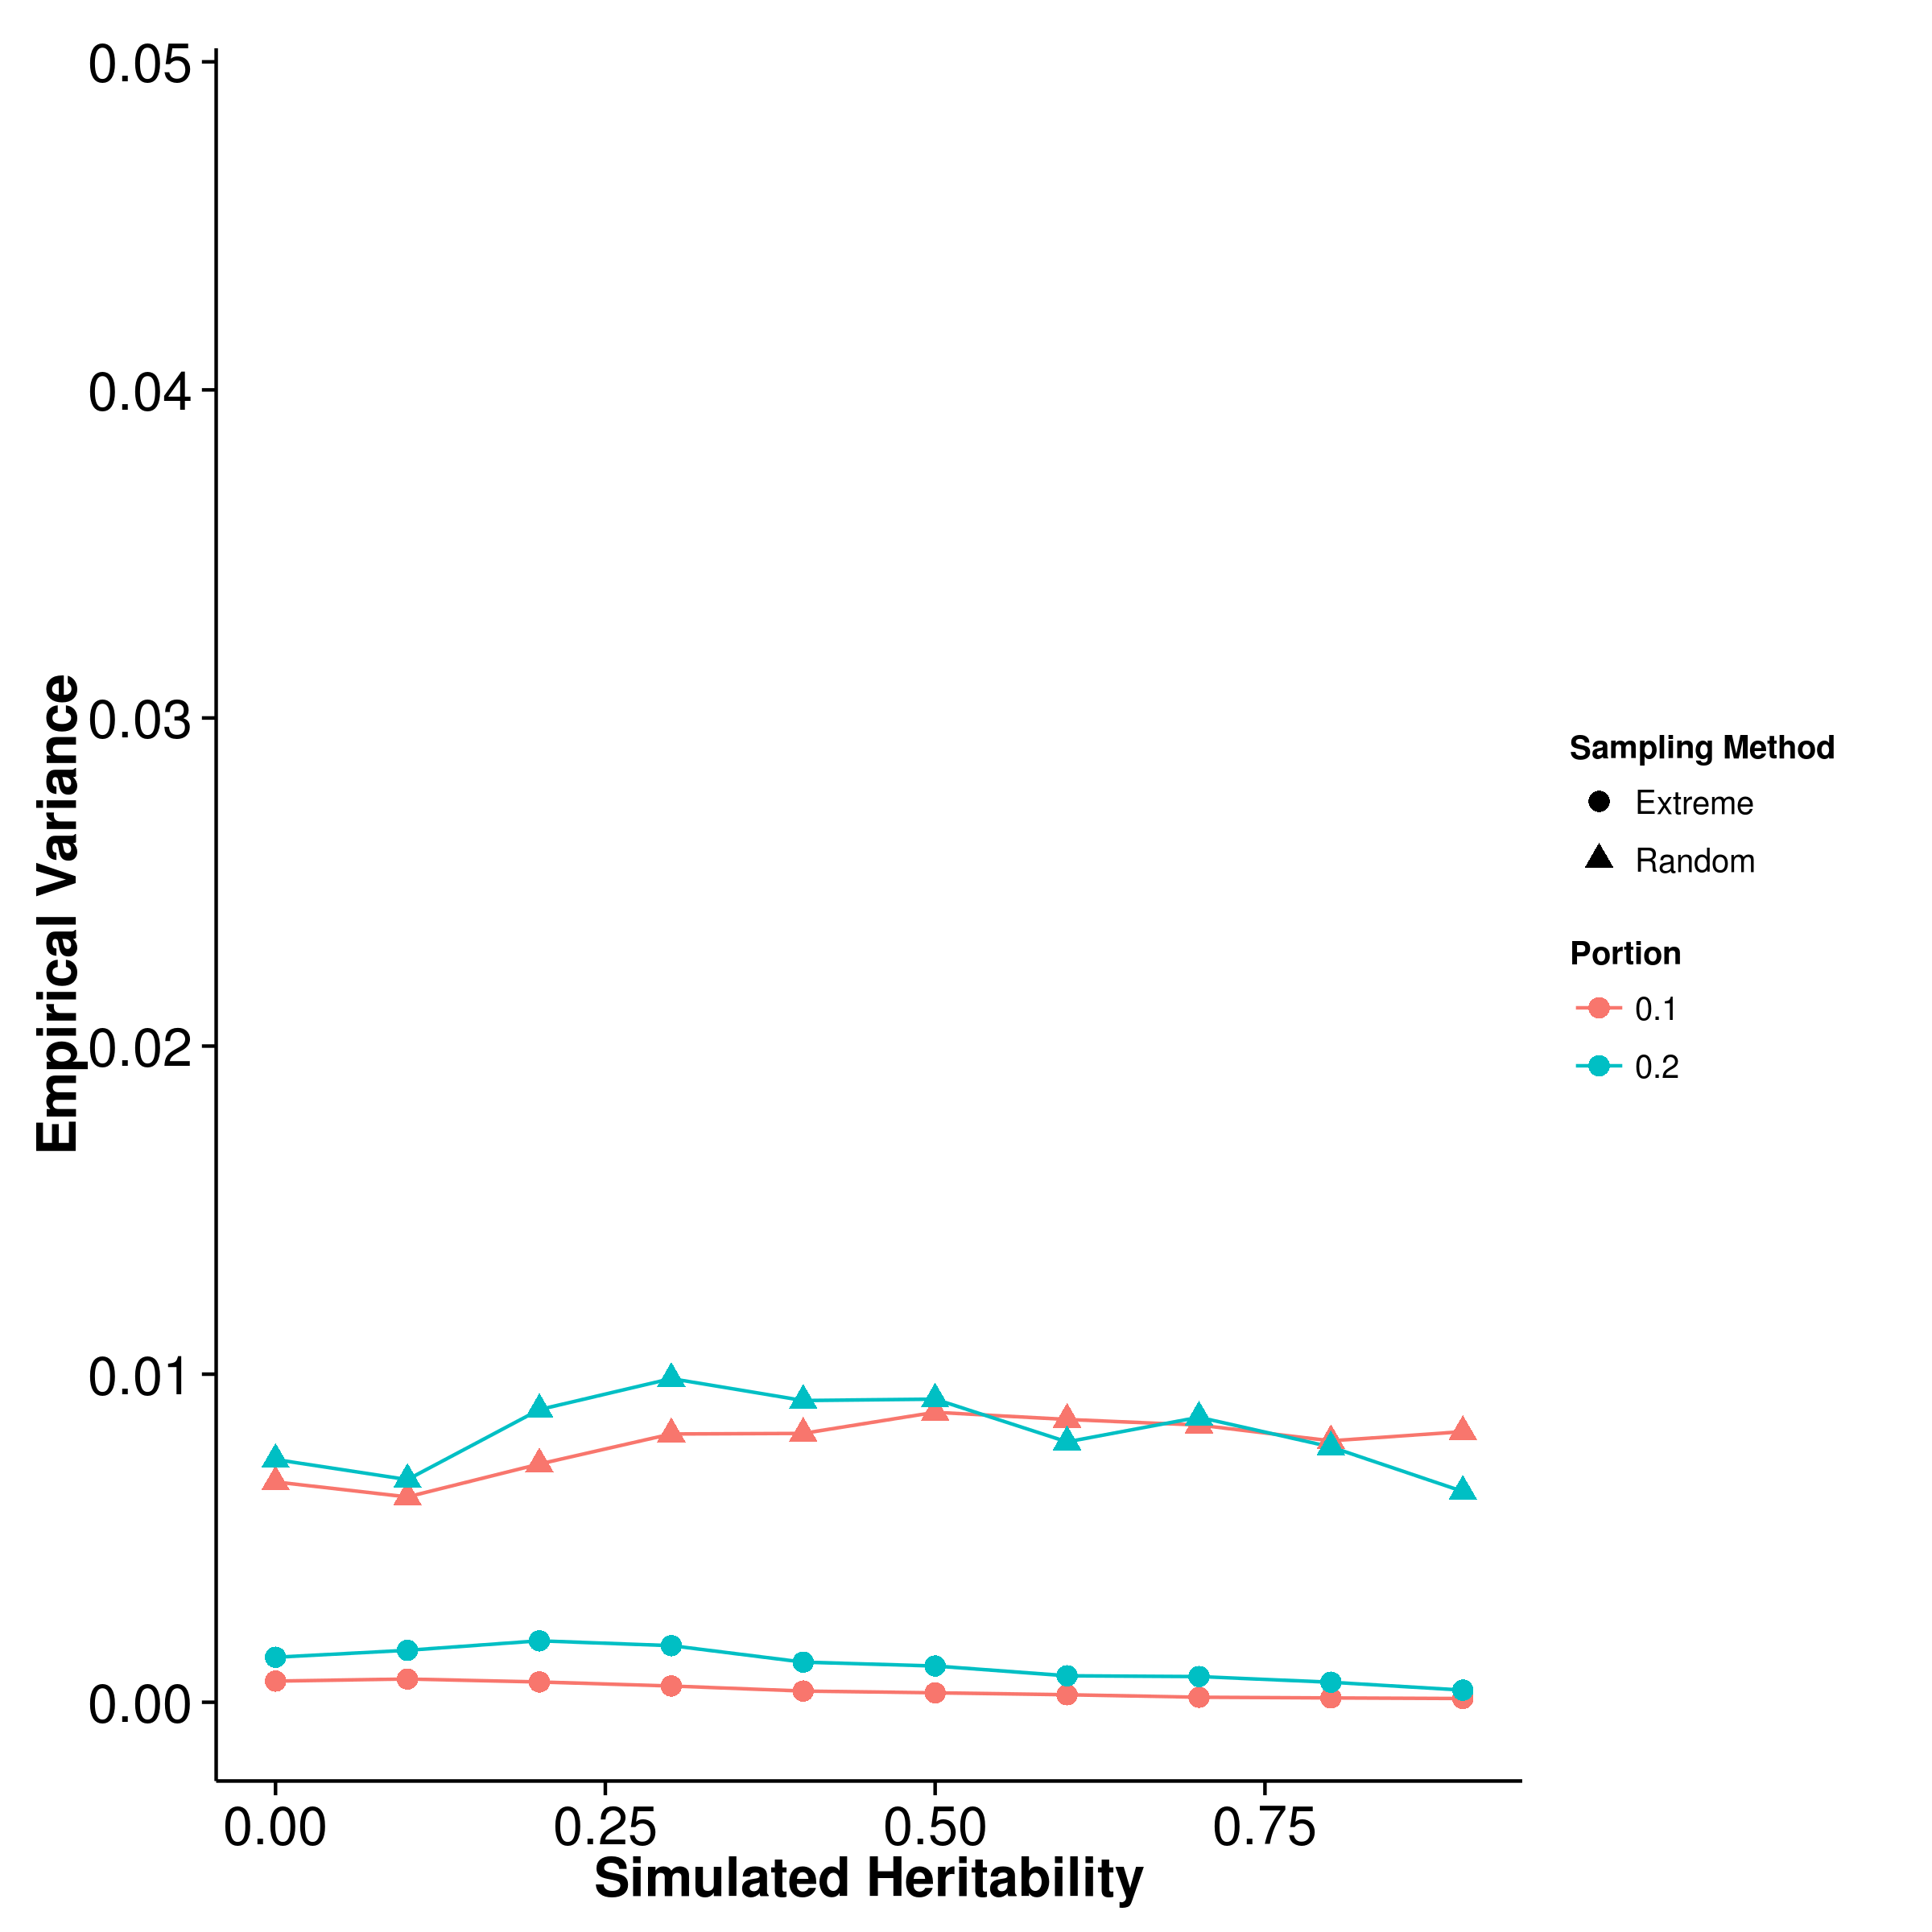
\includegraphics{figure/he_summary/pheno_extreme/gcta_extremeSelect_var.png}}
				\label{fig:gctaExVar}
			}\\
			\subfloat[LDSC with fix intercept]{
				\scalebox{.4}{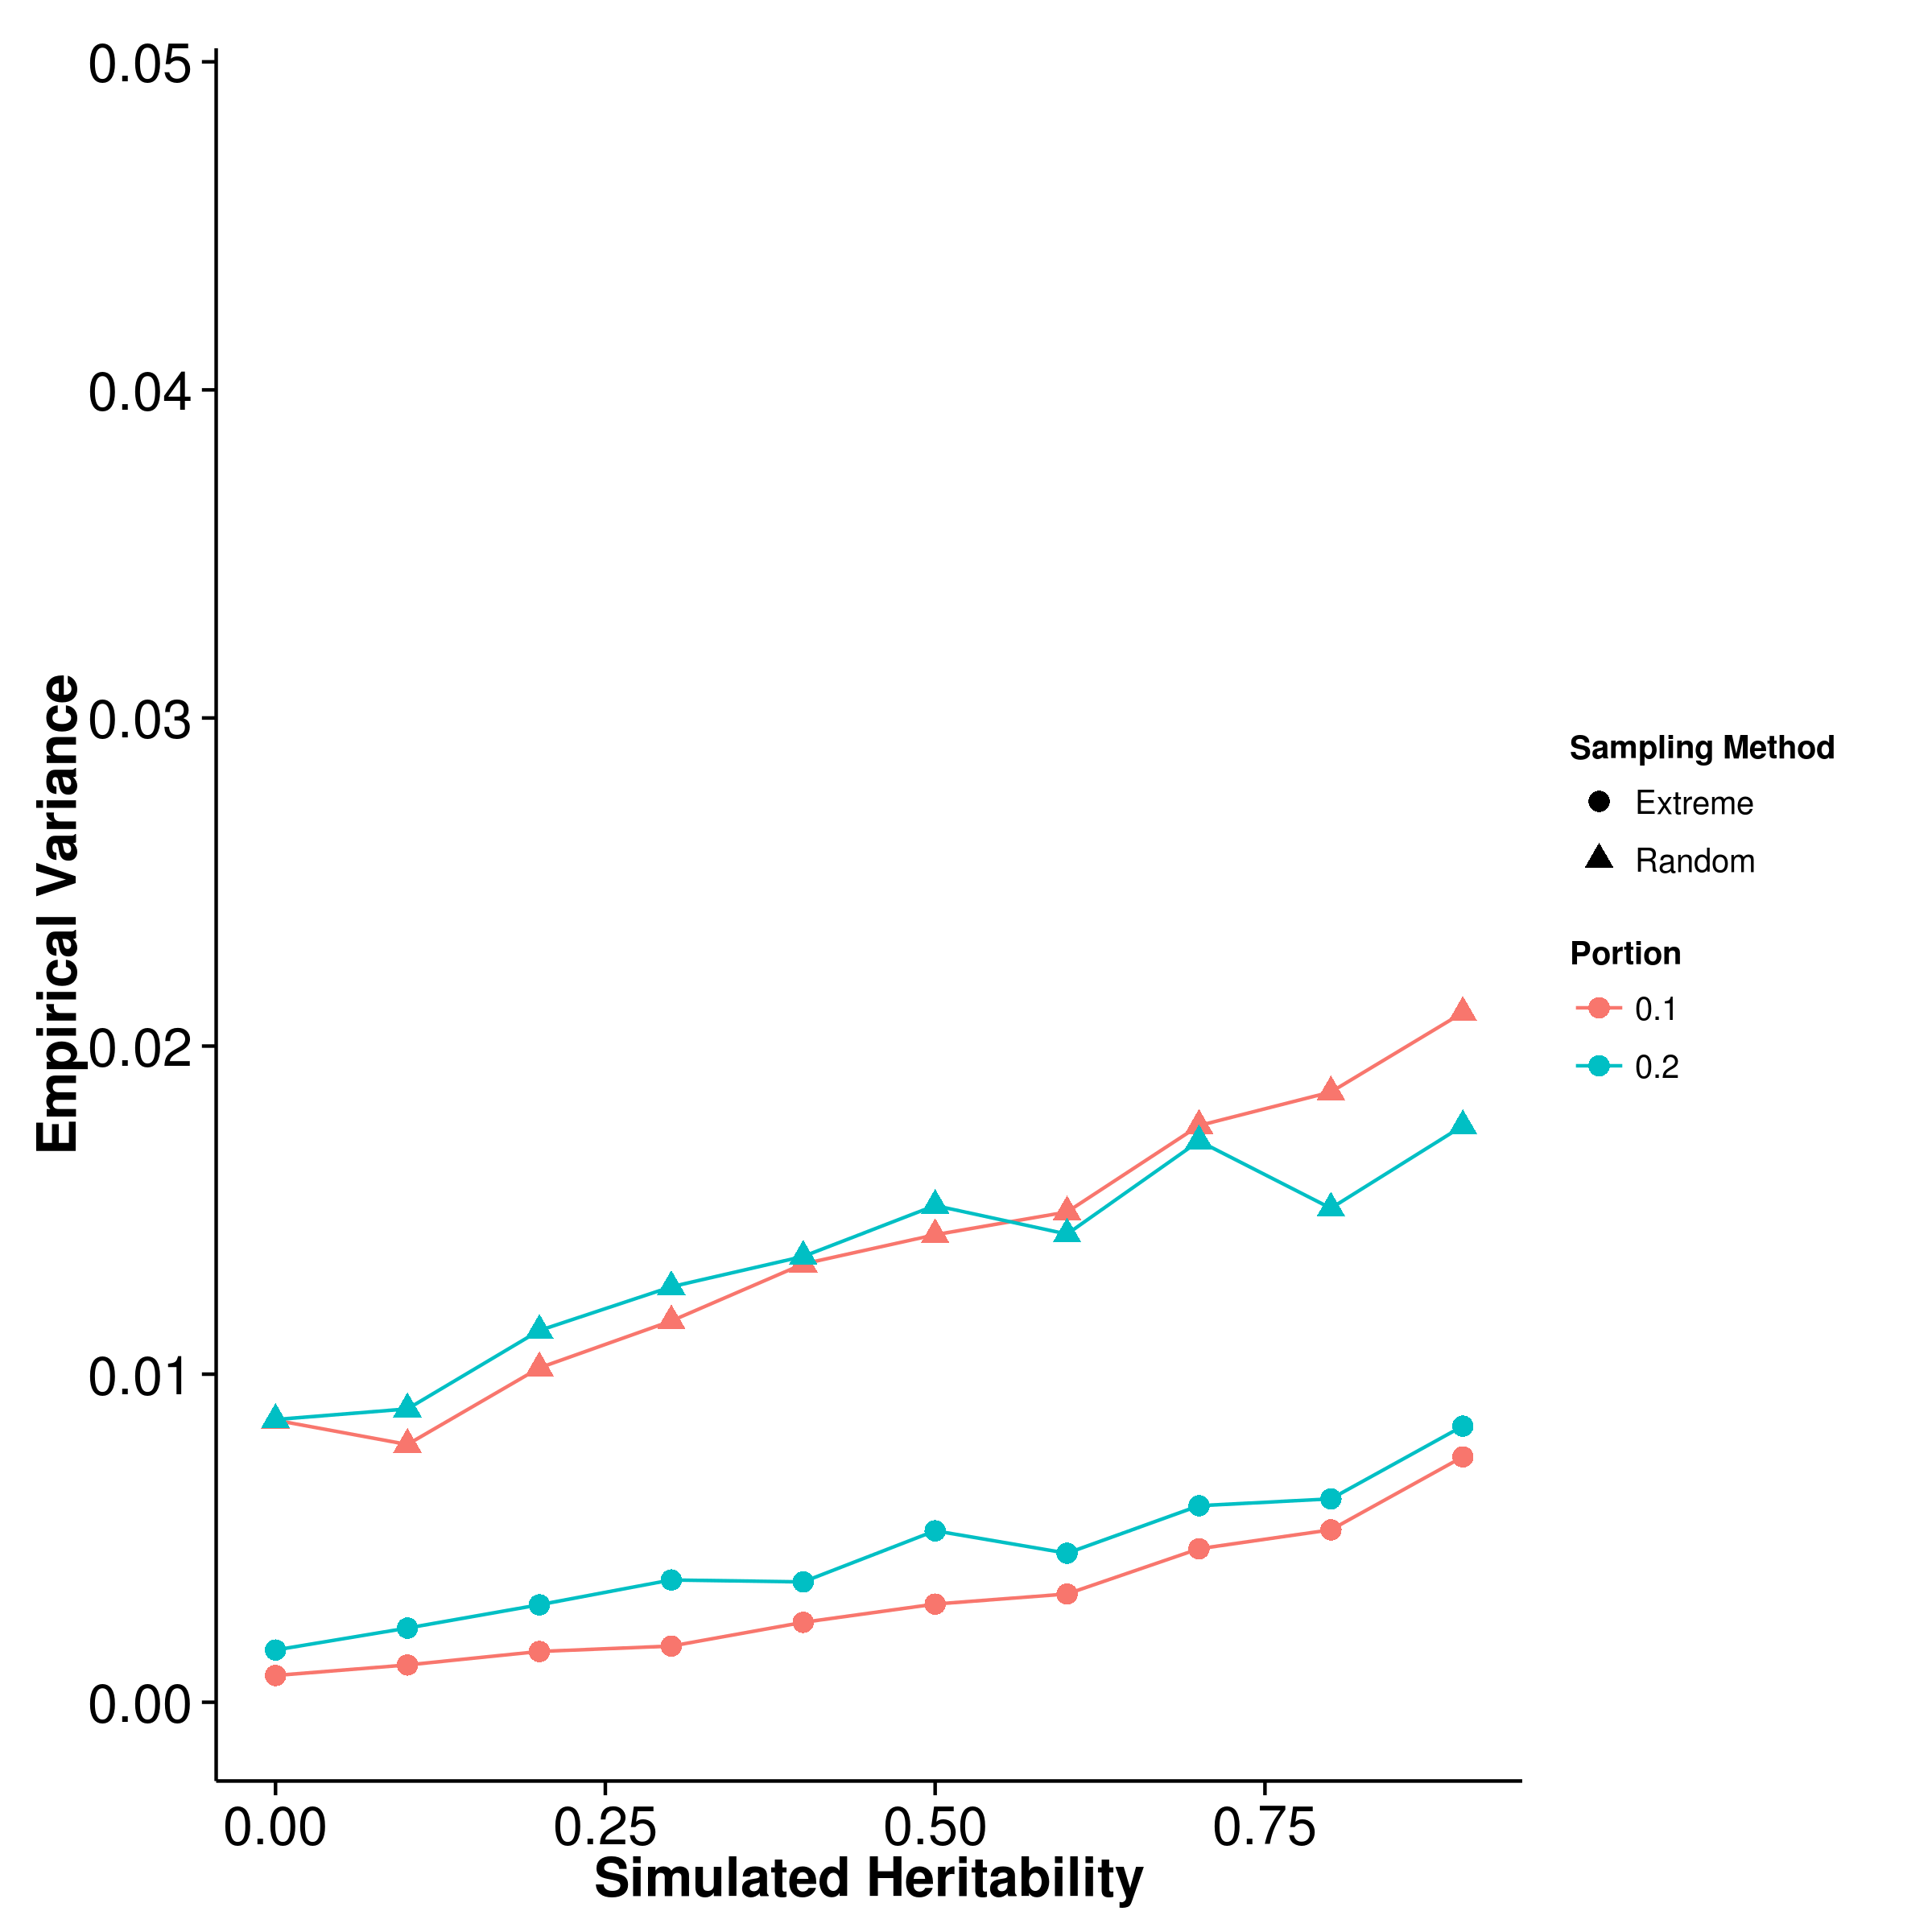
\includegraphics{figure/he_summary/pheno_extreme/ldsc_extremeSelect_var.png}}
				\label{fig:ldscEx}
			}
			\subfloat[LDSC with intercept estimation]{
				
				\scalebox{.4}{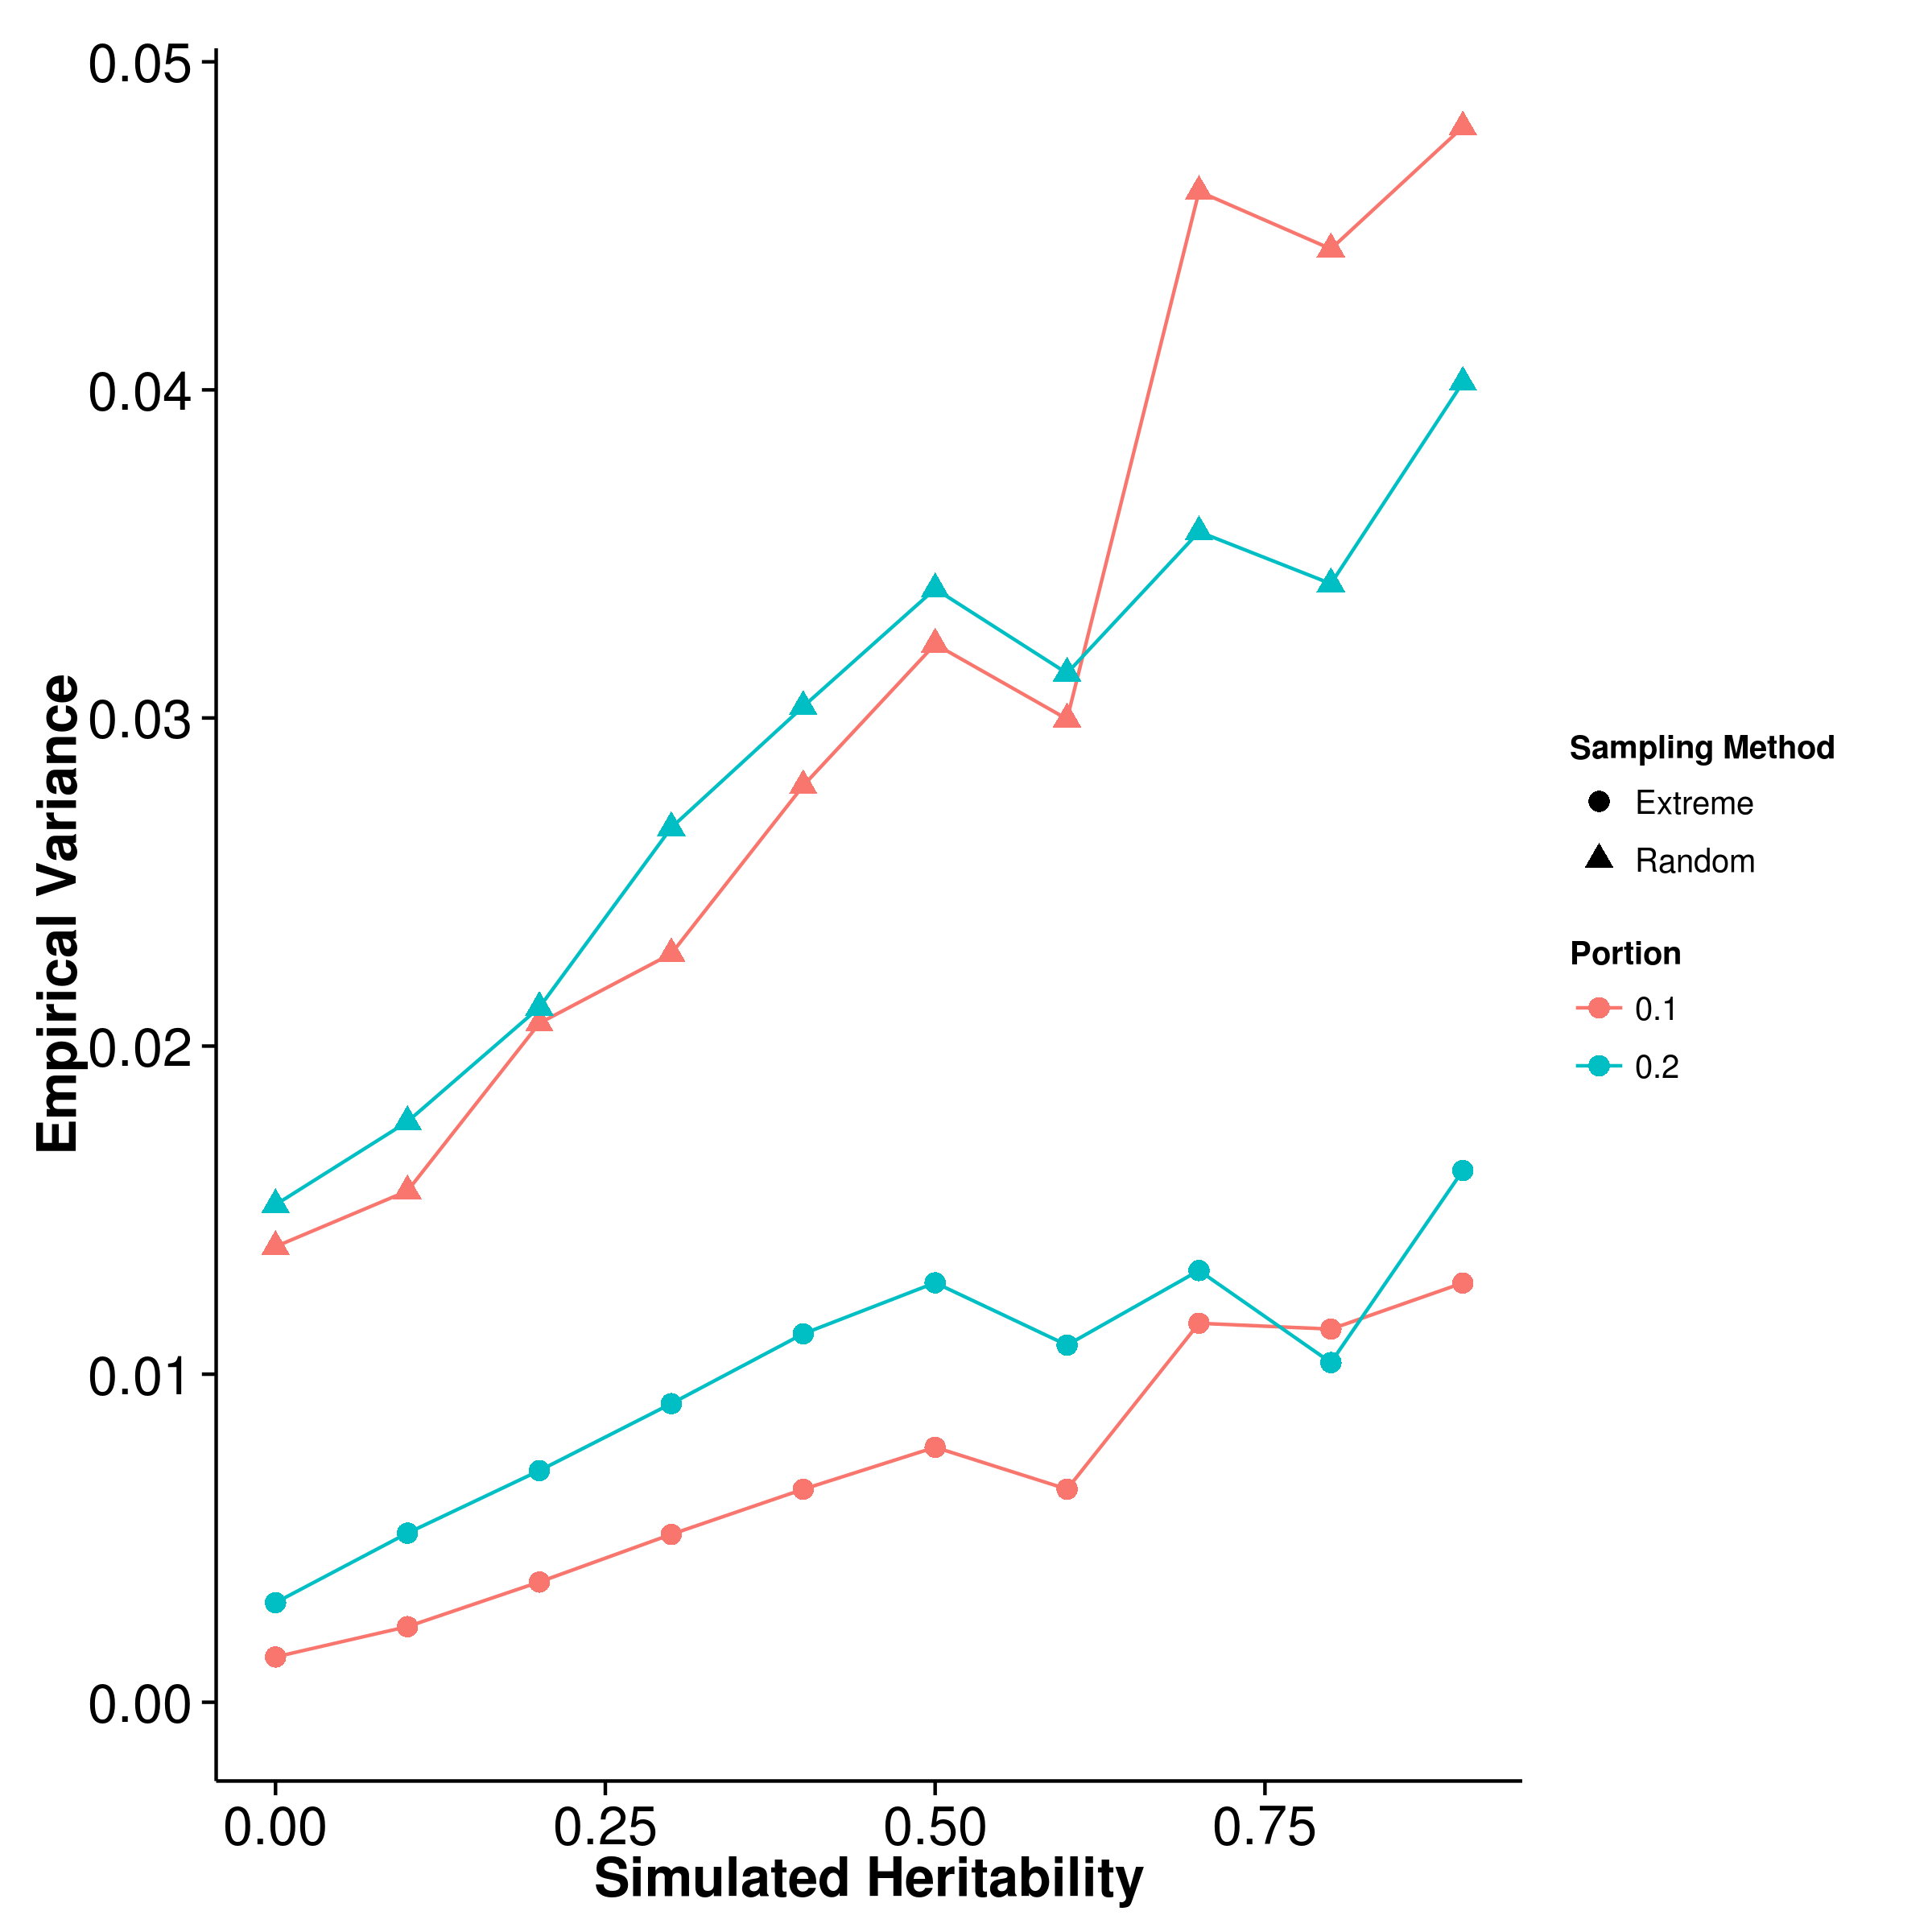
\includegraphics{figure/he_summary/pheno_extreme/ldscIn_extremeSelect_var.png}}
				\label{fig:ldscInExVar}
			}
			\caption[Variance of Extreme Phenotype Selection Simulation Results]
			{Variance of results from extreme phenotype simulation.
				It is obvious that when the extreme phenotype selection was performed, the empirical variance of all the algorithm decreases and is much smaller than the empirical variance of the estimation when random sampling was performed.
				We also compared the empirical variance of random sampling with those from quantitative trait simulation with 100 causal \glspl{SNP} and they are highly similar. 
			} 
			\label{fig:ExVar}
		\end{figure}
		
		
		\begin{figure}
			\centering
			\subfloat[SHREK]{
				\scalebox{.4}{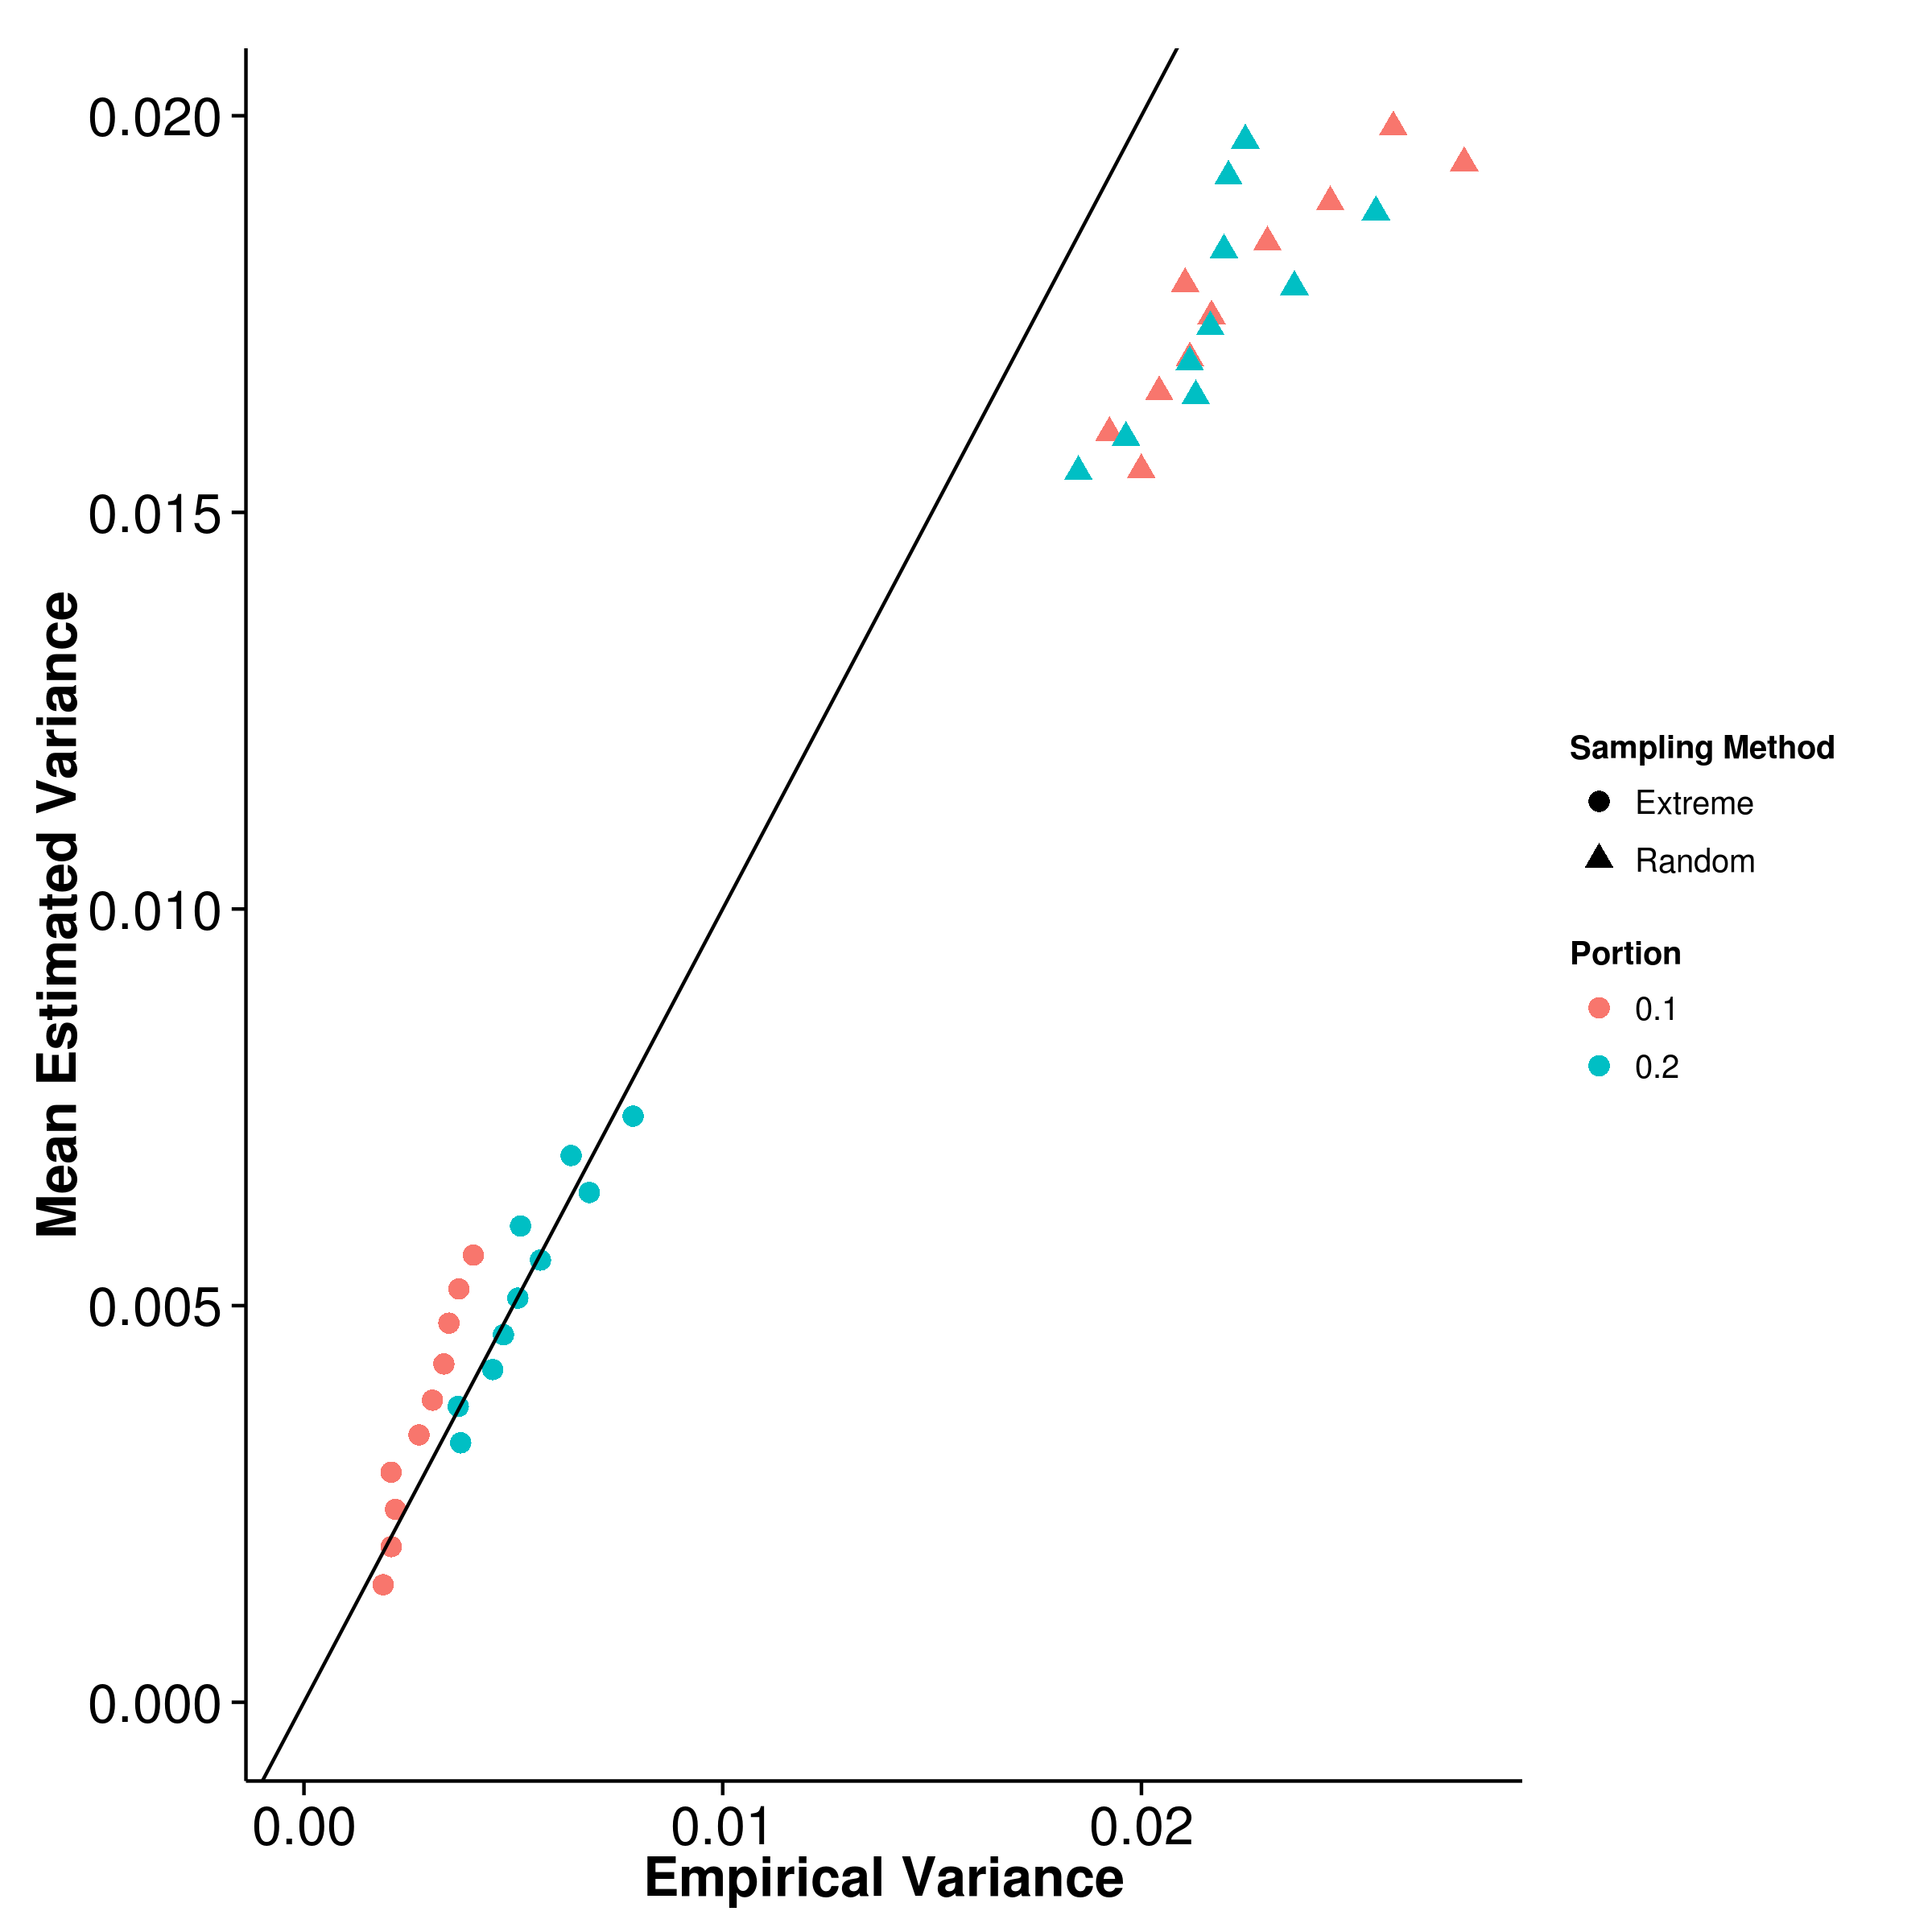
\includegraphics{figure/he_summary/pheno_extreme/shrek_extremeSelect_varCom.png}}
				\label{fig:shrekExVarCom}
			}
			\subfloat[GCTA]{
				\scalebox{.4}{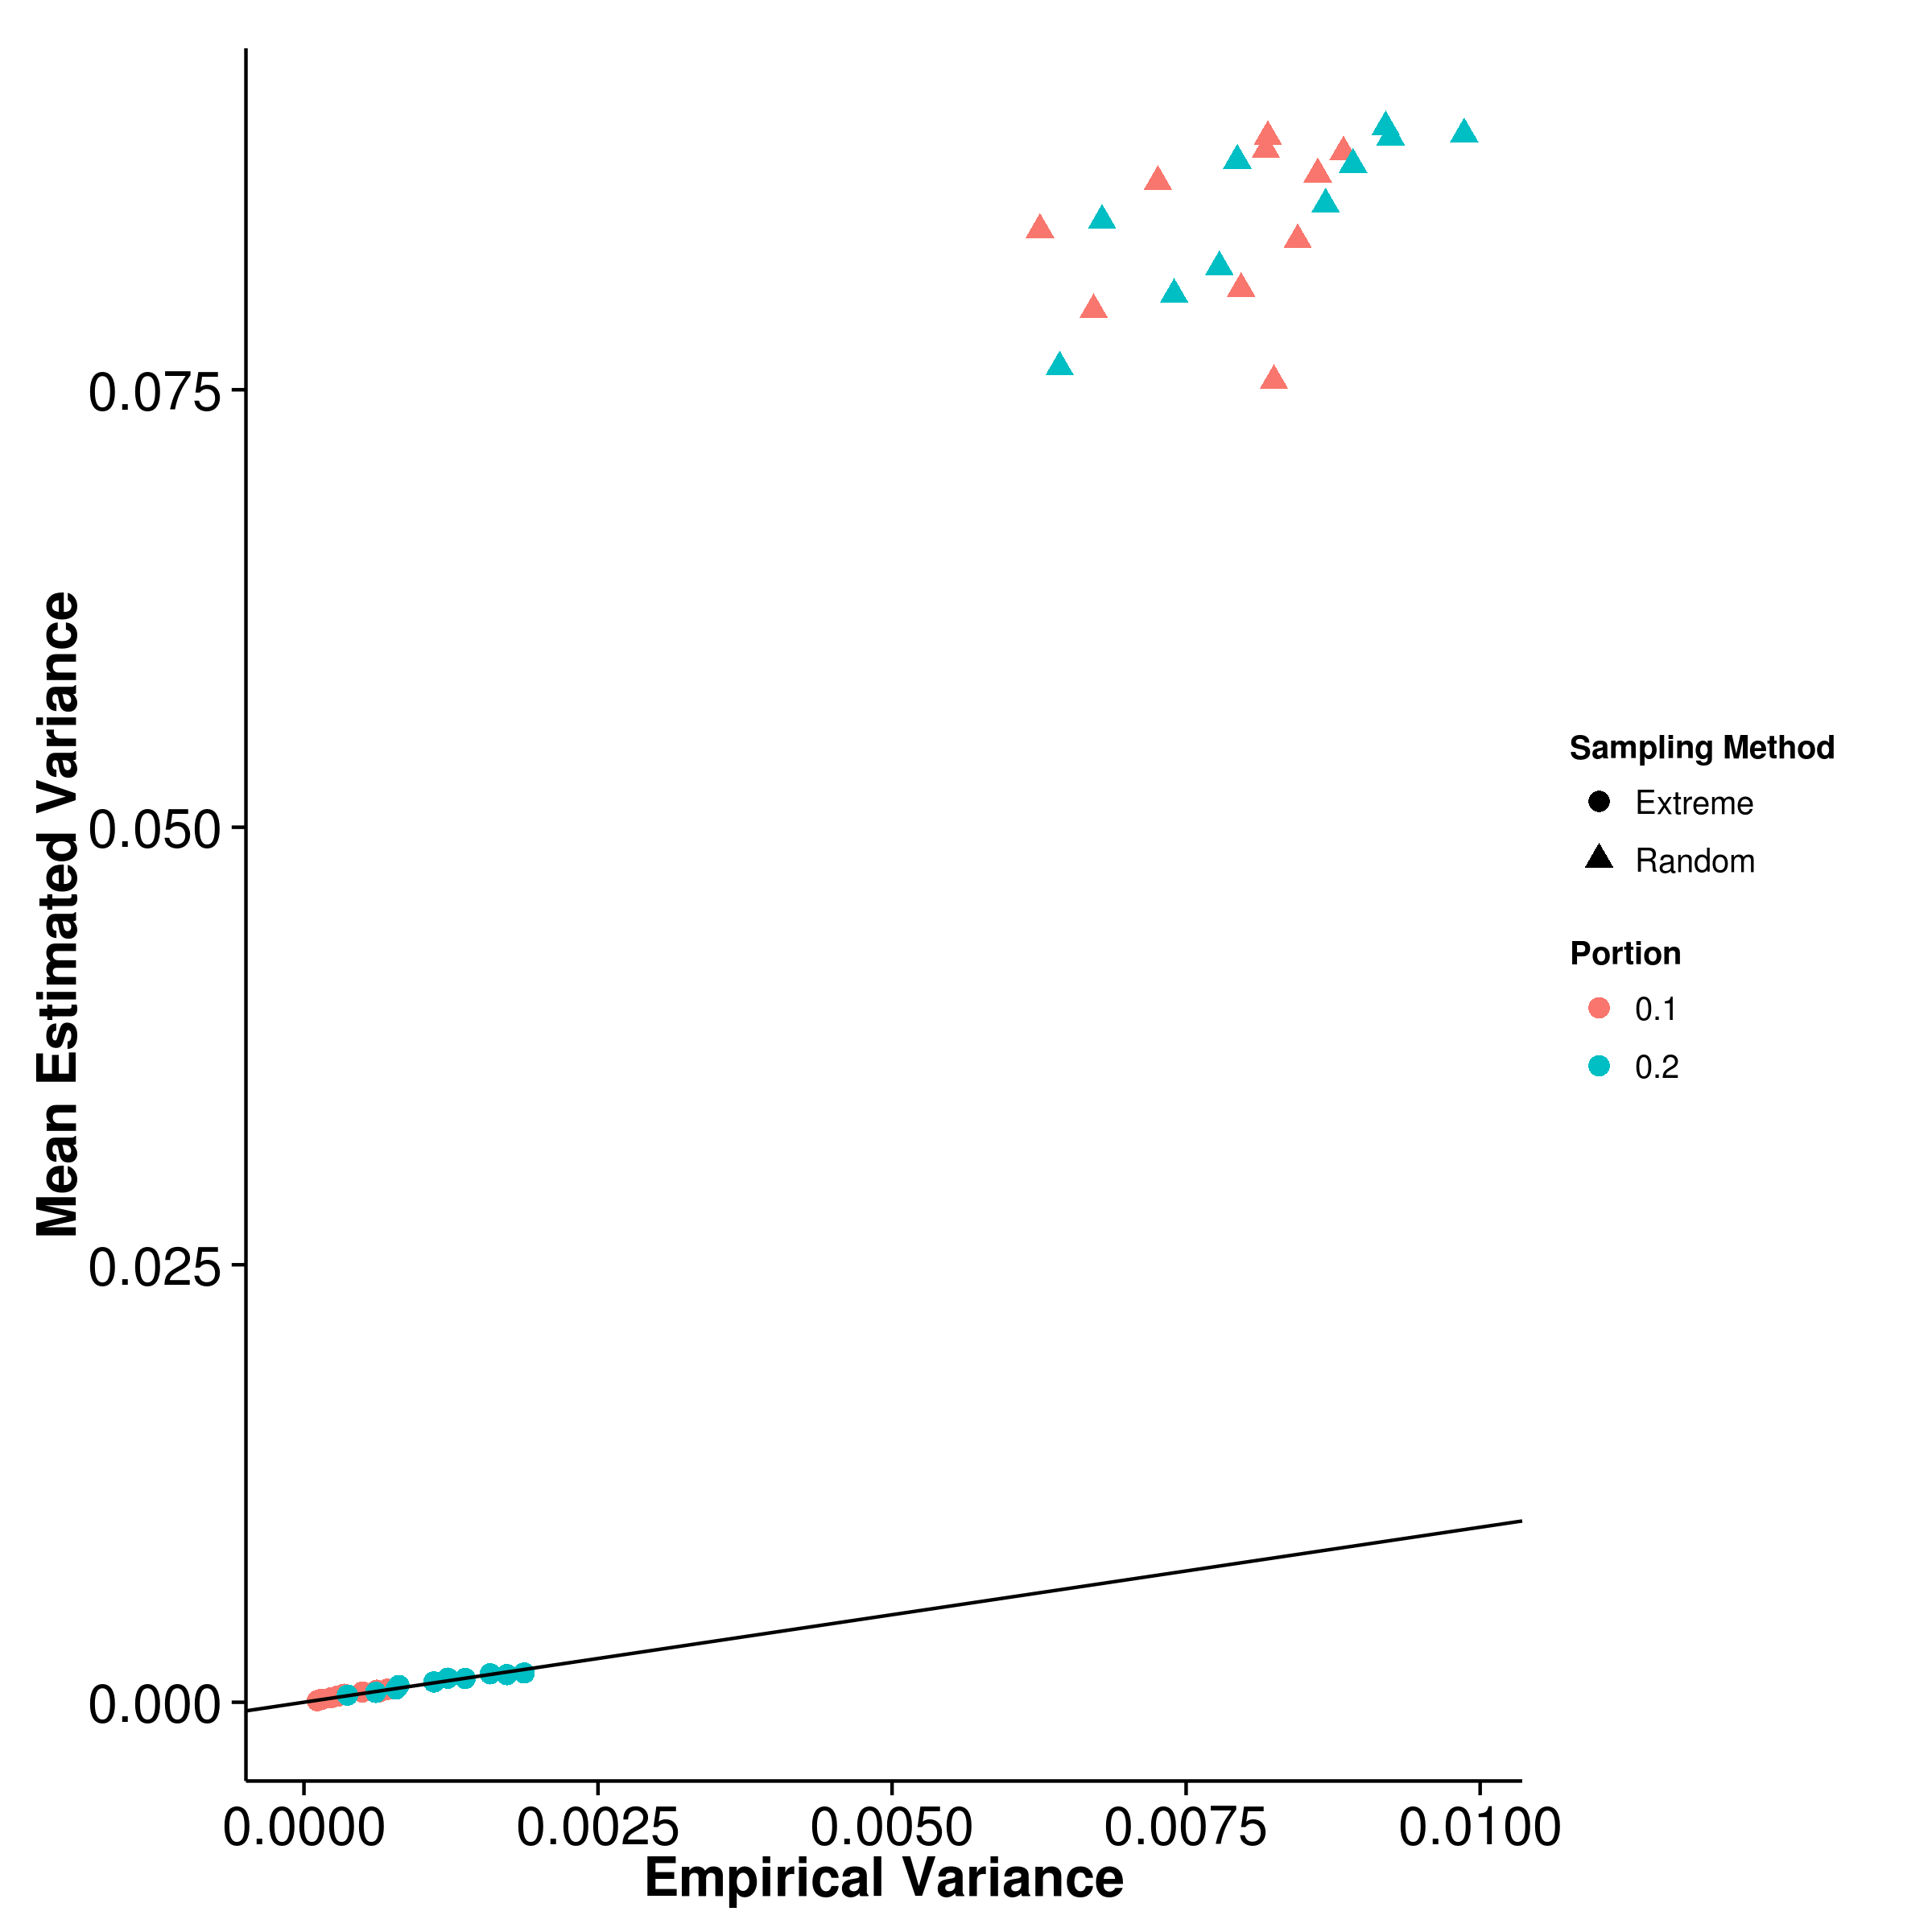
\includegraphics{figure/he_summary/pheno_extreme/gcta_extremeSelect_varCom.png}}
				\label{fig:gctaExVarCom}
			}\\
			\subfloat[LDSC with fix intercept]{
				\scalebox{.4}{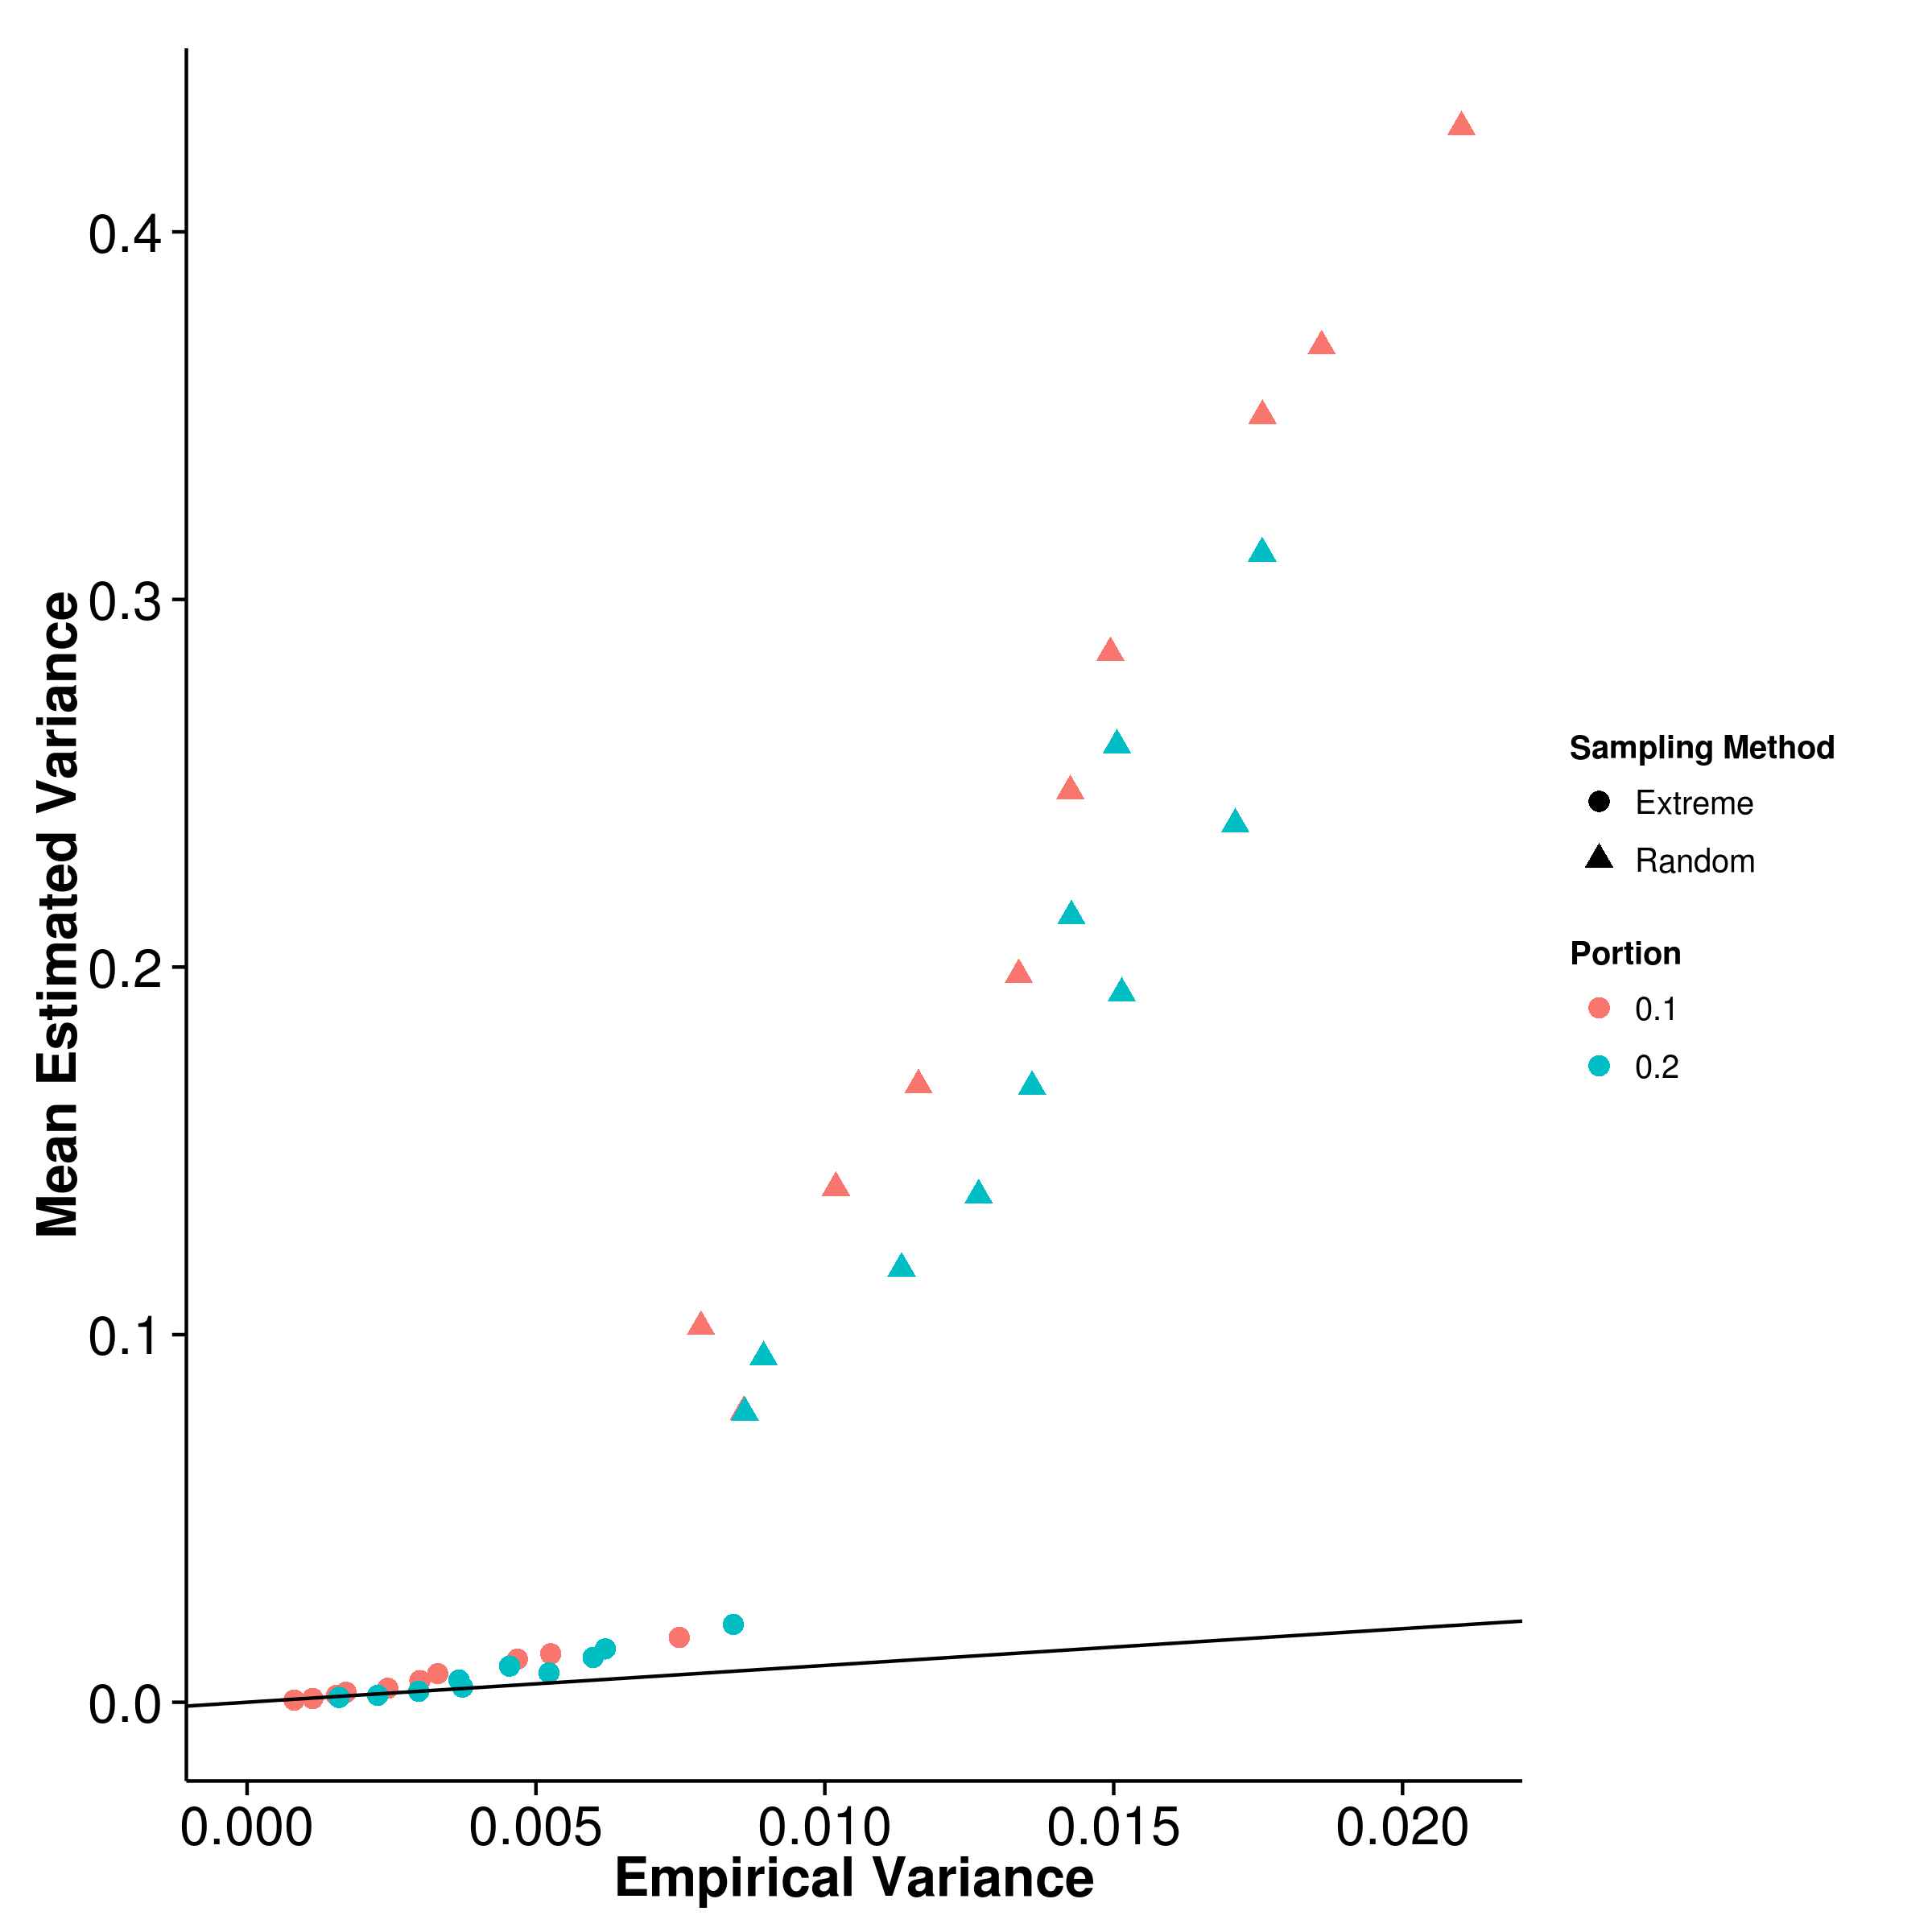
\includegraphics{figure/he_summary/pheno_extreme/ldsc_extremeSelect_varCom.png}}
				\label{fig:ldscExVarCom}
			}
			\subfloat[LDSC with intercept estimation]{
				
				\scalebox{.4}{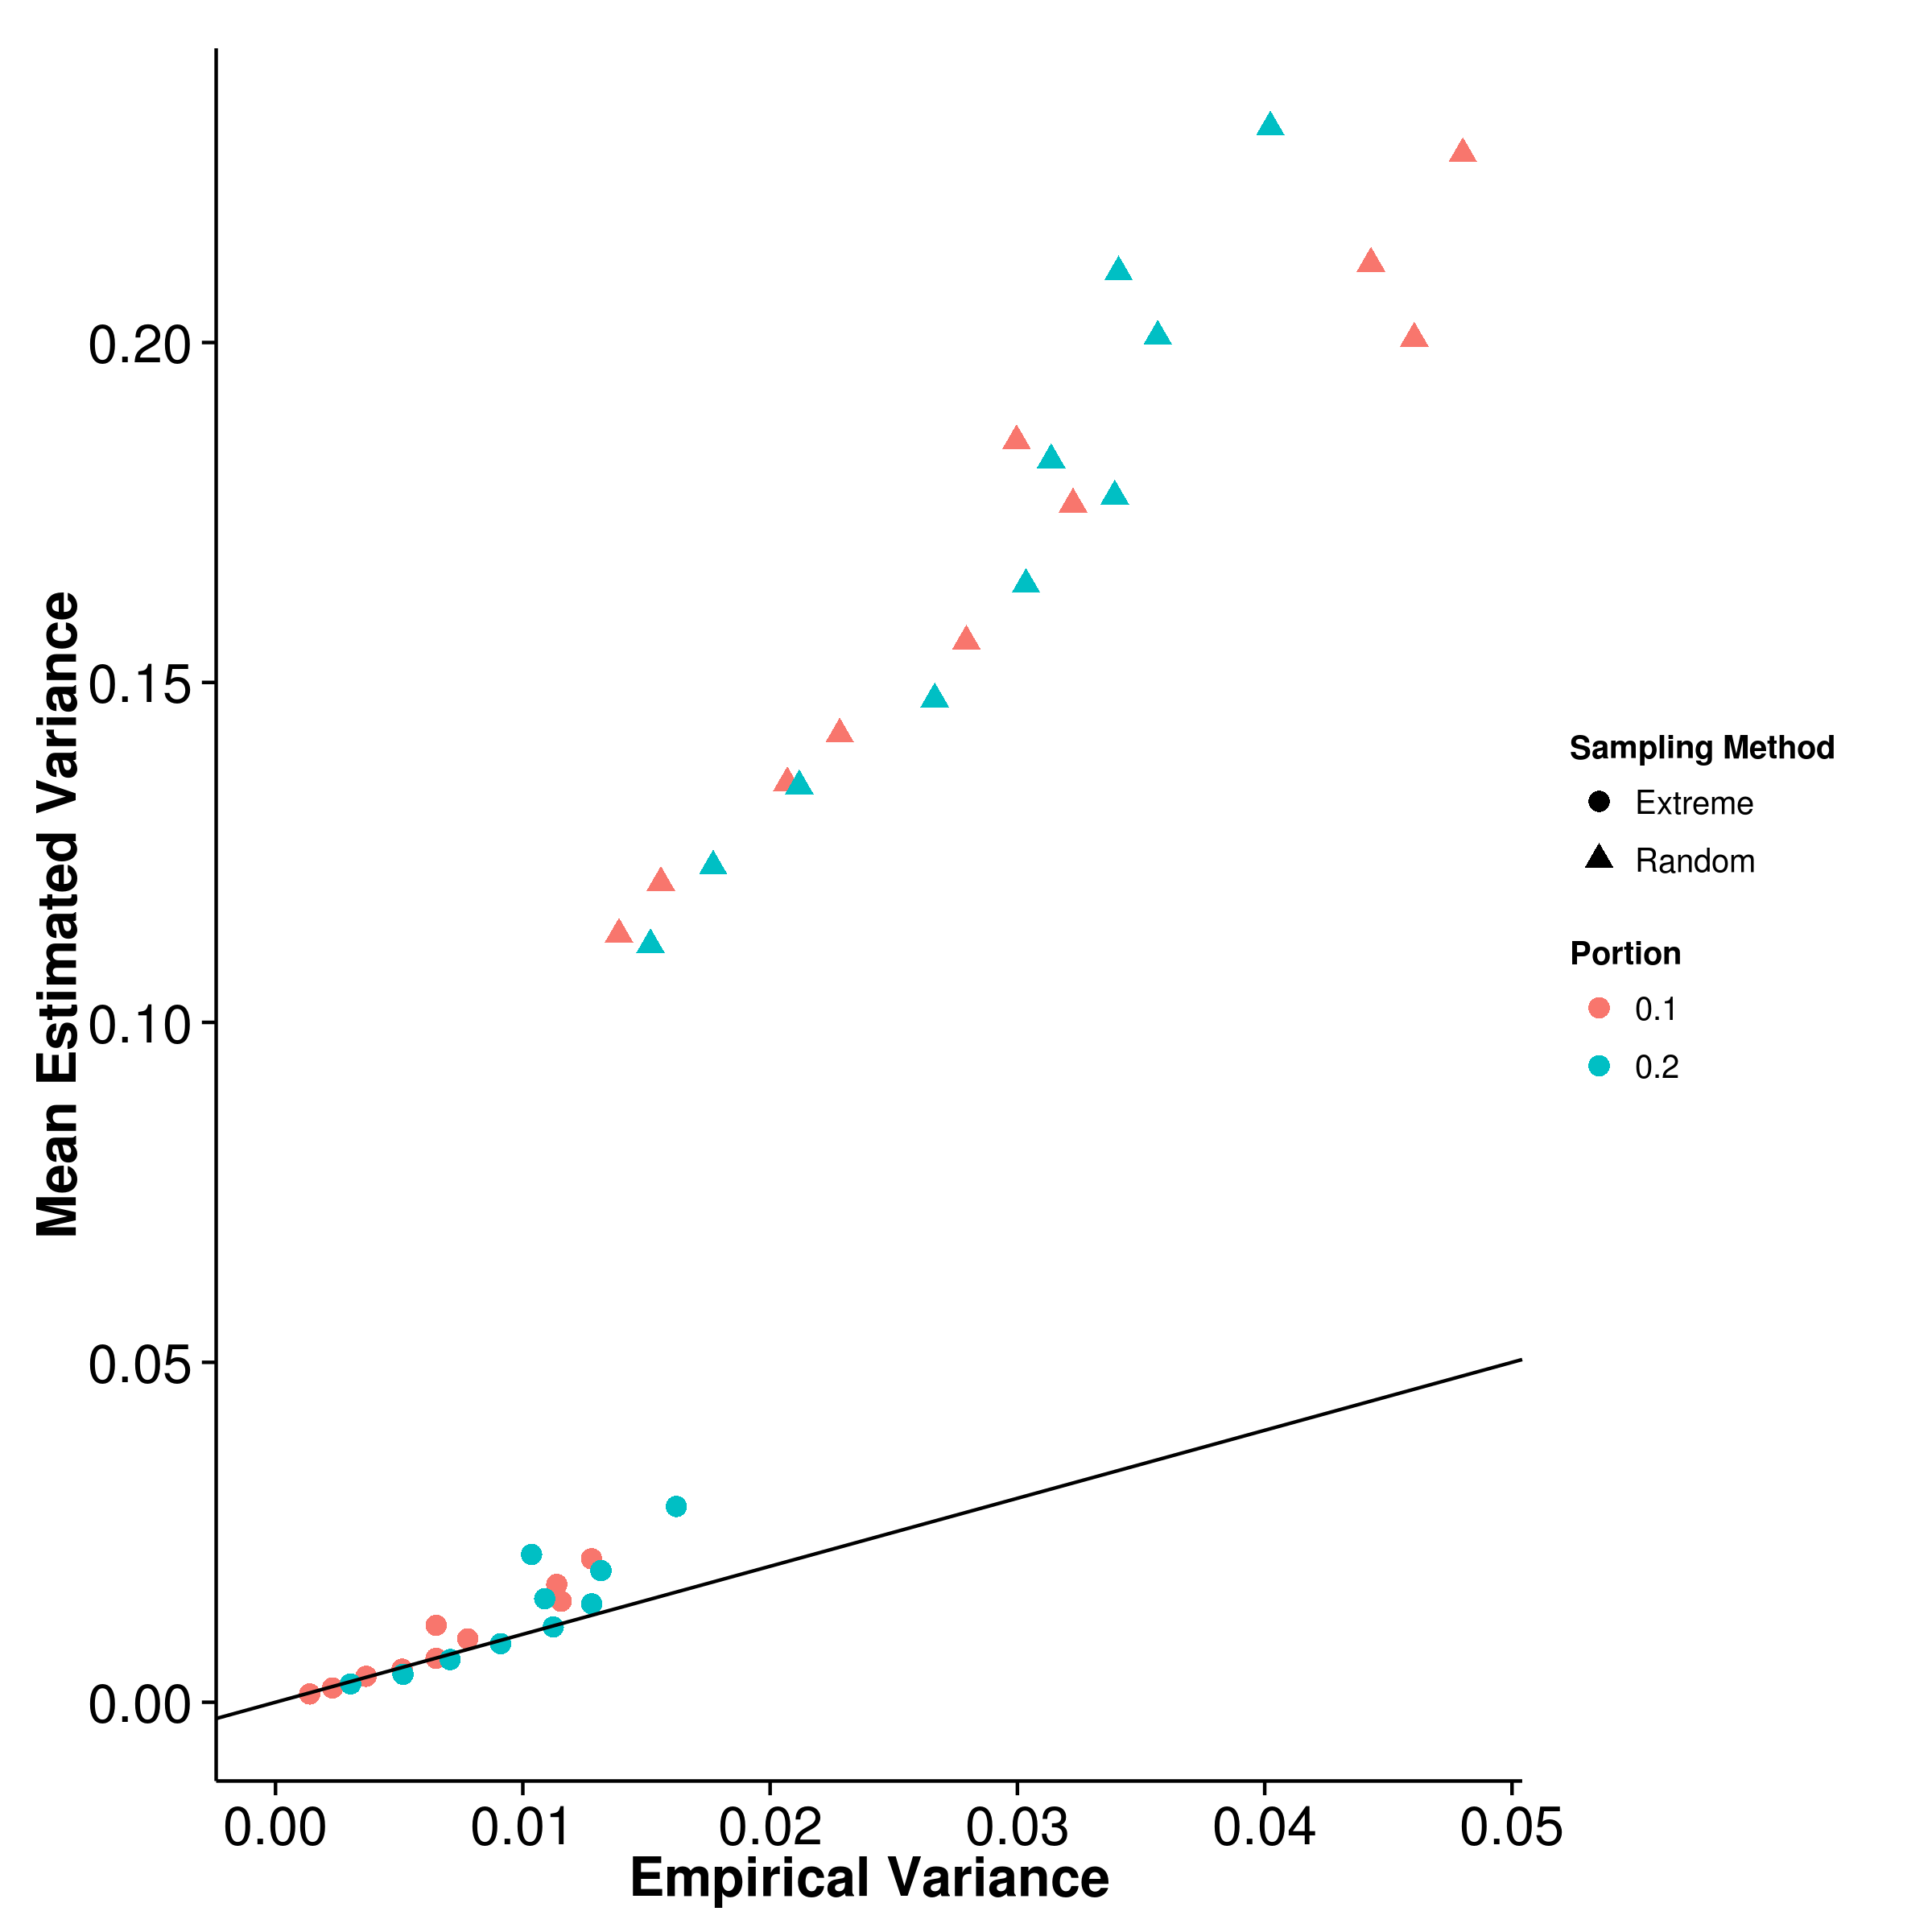
\includegraphics{figure/he_summary/pheno_extreme/ldscIn_extremeSelect_varCom.png}}
				\label{fig:ldscInExVarCom}
			}
			\caption[Estimation of Variance in Extreme Phenotype Selection]
			{Estimated variance of results from extreme phenotype selection when compared to empirical variance.
				Surprisingly, except for \gls{shrek}, the estimated variance from \gls{ldsc} and \gls{gcta} under the random sampling condition was much higher than the empirical variance. 
				It is much different from the estimated variance from the quantitative trait simulation and further investigations are required to understand this discrepancy.
				} 
			\label{fig:ExVarCom}
		\end{figure}